\chapter{Structure of $\Breal$ and $\Breal^{n}$}
\pagebreak[4]

\mysection{30}{Algebraic structure of $\Breal$ }
\subsection*{Remark on the Archimedean principle}
The Archimedean principle is sometimes stated as :\\
If $x,\,y\in \Breal$ with $y>0$, then $\exists n\in \Zed: (n-1)y\leq x < ny$.\\\\
On page $25$, we have \\\\
$\mathbf{30.6}$ \textbf{The least upper bound axiom for the real number system} $\mathbf{\Breal}$.\\
If $S$ is a nonempty subset of $\Breal$ and $S$ has an upper bound, then $S$ has a least upper bound in $\Breal$.\\\\
It is strange that  the author first gives the Archimedean principle as a principle (aka Axiom ?) and afterwards $\mathbf{30.6}$ as an axiom as the Archimedean principle can be proved with this axiom. \\\\
\textbf{Proof} (by contradiction):\\
Be arbitrary $x,\, y\in \Breal$ with $y> 0$. Suppose that we have $py\leq x$ is true for all $p\in \Zed$. Be $A$ the subset of $\Breal$ with all the real numbers $py$ as elements. From axiom $\mathbf{30.6}$ we know that $A$ has a least upper bound with $x$ as an upper bound. Be $\xi= lub(A)$. As we have $y>0$, then $\xi -y$ is not an upper bound of $A$.  This mean that there is a $p$ such that $py>\xi -y$. Hence, $ (p+1)y>\xi$. Thus $\xi$ can not be a upper bound of $A$, and we have a contradiction. Hence, there must be a $p\in \Zed$ for which $py>x$.
\newpage
\renewcommand{\thesubsection}{\thesection.\arabic{subsection}}
\setcounter{subsection}{0}
\subsection{}
%\subsubsection{}{}
\begin{tcolorbox}
Explain by example why it is that the system of all rational numbers does not satisfy the least upper bound axiom.
\end{tcolorbox}
Be $A\subset\Qiuu$ such that $A=\{x^2\leq 2,\, x\in \Qiuu\}$. $A$ has upper bounds (e.g.  $sup(A)=2$). This set can be re-expressed as $A= (-\sqrt{2},\sqrt{2})$ and has no $l.u.b.(A)$ as $\sqrt{2}\not \in \Qiuu$.
$$\blacklozenge$$

\subsection{}
%\subsubsection{}{}
\begin{tcolorbox}
Prove that the least upper bound property implies the following: If $S$ is a nonempty subset of real numbers that has a lower bound, then $S$ has a greatest lower bound. 
\end{tcolorbox}
Suppose $S$ is a nonempty subset of real numbers that has a lower bound $\mathbcal{s}$. For all $x\in S$ we have $\mathbcal{s}\leq x$. Let's define a new set $\hat{S}$ with $\hat{S}=\{2\mathbcal{s}-x: x\in S\}$. Then, $\mathbcal{s}$ is an upper bound for $\hat{S}$. By the upper bound axiom for real number, we have a $\mathbcal{\hat{s}}= l.u.b.(\hat{S})$ and we have $2\mathbcal{s}-x\leq \mathbcal{\hat{s}}$ for all $x\in S$. And thus, $$2\mathbcal{s}- \mathbcal{\hat{s}}\leq x$$
for all $x\in S$.\\
$2\mathbcal{s}- \mathbcal{\hat{s}}$ is a $g.l.b.(A)$ as, suppose we would have a $\epsilon>0$ such that  $2\mathbcal{s}- \mathbcal{\hat{s}}+\epsilon \leq x$ and thus $\underbrace{2\mathbcal{s}-x}_{\in\hat{S}} \leq \mathbcal{\hat{s}}-\epsilon$ for all $\hat{x}\in \hat{S}$. We get a contradiction as we would have $\mathbcal{\hat{s}}-\epsilon$ as an upper bound which is smaller than $l.u.b.(\hat{S})$.
$$\blacklozenge$$

\subsection{}
%\subsubsection{}{}
\begin{tcolorbox}
Let $S = \left\{x:x=1-\frac{1}{n},\, n\in\Pee\right\}$. Find $l.u.b. (S)$ and $g.l.b. (S)$ if they exist. 
\end{tcolorbox}
$$ $$ 
For $n=1$ we have $x=0$ and thus $g.l.b(S)=0$.\\\\
For $n\rightarrow +\infty $ we have $x\rightarrow 1$ and thus $l.u.b(S)=1$.
$$\blacklozenge$$

\subsection{}
%\subsubsection{}{}
\begin{tcolorbox}
Let $f:\Breal\rightarrow \Breal$  be given by $f (x)=x^3$. Find the $l.u.b. (f [\{x: 0 < x < 1\}])$. \\
Find $l.u.b. (f [\{x:0\leq x\leq 1\})$. 
\end{tcolorbox}
$$ $$ 
$l.u.b. (f [\{x: 0 < x < 1\}])= 1$.\\\\
$l.u.b. (f [\{x:0\leq x\leq 1\})= 1$
$$\blacklozenge$$

\subsection{}
%\subsubsection{}{}
\begin{tcolorbox}
Suppose that $f: \{x :0 < x\}\rightarrow\Breal$ is given by $f (x)= \frac{1}{x}$  for $0 < x$. Does $f [\{x : 0 < x\}]$ have a $l.u.b.$? Does it have a $g.l.b.$? 
\end{tcolorbox}
$$ $$ 
$l.u.b. (f [\{x : 0 < x\}])$ does not exist.\\\\
$g.l.b. (f [\{x : 0 < x\}])=0$.
$$\blacklozenge$$

\subsection{}
%\subsubsection{}{}
\begin{tcolorbox}
Give an example of a function $f$ defined on a closed interval $S$ such that $l.u.b. (f [S])$ exists but $f$ does not attain a maximum value on $S$.
\end{tcolorbox}
Consider $f:\Breal_{[0,1]}\rightarrow \Breal$ such that $f=\left\{\frac{1-a^{-\frac{x}{1-x}}}{1+a^{-\frac{x}{1-x}}}:x\in \Breal_{[0,1]},\, a>1 \right\}$ with $l.u.b. (f [S])=1\not\in f [S]$.
$$\blacklozenge$$

\subsection{}
%\subsubsection{}{}
\begin{tcolorbox}
Prove the following statement: If $a = l.u.b. (A)$, then for each $\epsilon > 0$ , there is an $x \in  A$ such that $a-\epsilon < x \leq a$. State and prove an analogous proposition for $g.l.b. (A)$. 
\end{tcolorbox}
Suppose for a given $\epsilon$,  $\not\exists\, x\in A:\, a-\epsilon < x$, then, $x\leq a-\epsilon$. Thus $a-\epsilon$ is a lower bound which is smaller than $l.u.b.(S)$. We have a contradiction and thus $\forall\epsilon\in\Breal, \exists\, x\in A:\, a-\epsilon < x \leq a$.\\\\
For $b= g.l.b. (A)$, the statement becomes $$\forall\epsilon\in\Breal, \exists\, x\in A:\, b\leq  x < b+\epsilon$$
Suppose for a given $\epsilon$,  $\not\exists\, x\in A:\, x < b+\epsilon$, then, $x \leq b+\epsilon$. Thus $b+\epsilon$ is a upper bound which is greater than $g.l.b.(S)$. We have a contradiction and thus $\forall\epsilon\in\Breal, \exists\, x\in A:\, b\leq  x < b+\epsilon$.
$$\blacklozenge$$

\subsection{}
%\subsubsection{}{}
\begin{tcolorbox}

Prove that if $A$ is a nonempty bounded set of real numbers then $g.l.b. (A) \leq l.u.b. (A)$. For what kind of set $A$ is $g.l.b. (A) =l.u.b. (A)$? 
\end{tcolorbox}
$A$ is bounded, hence by the upper bound property and its corollary (see Exercise 2.30.2) then $A$ has both a $l.u.b.(A)$  and a $g.l.b.(A)$. This mean that for every $x\in A$ we have $l.u.b.(A)\leq x\leq g.l.b.(A)$ and thus $l.u.b.(A)\leq g.l.b.(A)$\\\\
We can have $g.l.b. (A) =l.u.b. (A)$ when $A$ is a singleton, i.e. $A=\{x\}$. E.g. $A=f[\Breal]$ with $f=\{c\}$ with $c$ a constant, has $g.l.b. (A) =l.u.b. (A)=c$ .
$$\blacklozenge$$



\subsection{}
%\subsubsection{}{}
\begin{tcolorbox}
Prove that if $A$ and $B$ are nonempty subsets of $\Breal$ and $A \subset B$, then $g.l.b. (B) \leq g.l.b. (A)\leq  l.u.b. (A) \leq l.u.b. (B)$. 
\end{tcolorbox}
From $\mathbf{2.30.8}$ we know that $l.u.b.(A)\leq g.l.b.(A)$ and $l.u.b.(B)\leq g.l.b.(B)$. \\\\
Suppose we have $g.l.b.(A)< g.l.b.(B)$. This implies that $\exists x\in A: x\not \in B$. We have a contradiction as $A\subset B$ and thus we must have $g.l.b.(B)\leq g.l.b.(A)$.\\
In the same vein, suppose we have $l.u.b.(B)< l.u.b.(A)$. This implies that $\exists x\in A: x\not \in B$. We have a contradiction as $A\subset B$ and thus we must have $l.u.b.(A)\leq l.u.b.(B)$. \\
Putting this all together we get indeed
$$g.l.b. (B) \leq g.l.b. (A)\leq  l.u.b. (A) \leq l.u.b. (B)$$
$$\blacklozenge$$
\newpage

\mysection{31}{ Distance between two points in $\Breal$}

\renewcommand{\thesubsection}{\thesection.\arabic{subsection}}
\setcounter{subsection}{0}
\subsection{}
%\subsubsection{}{}
\begin{tcolorbox}
Verify the properties stated in $\mathbf{31.2}$
\end{tcolorbox}
$\mathbf{31.2(a)}$ and $\mathbf{31.2(b)}$ are trivial as $d(x,y)=|x-y|$.\\\\
$\mathbf{31.2(c)}$:\\
We consider 4 possibilities (the cases $a=b$ or $b=c$ are excluded as in that case $d(a,b)$ or $d(b,c)$ are zero).\\
i) $a<b$ and $b<c$. Then, 
$$d(a,c)= |a-b+b-c| = |-|a-b|-|b-c||= | |a-b|+|b-c| |= d(a,b)+d(b,c)$$
ii) $a<b$ and $b>c$. Then, 
$$d(a,c)= |a-b+b-c| = |-|a-b|+|b-c||< | |a-b|+|b-c| |= d(a,b)+d(b,c)$$
ii) $a>b$ and $b<c$. Then, 
$$d(a,c)= |a-b+b-c| = ||a-b|-|b-c||< | |a-b|+|b-c| |= d(a,b)+d(b,c)$$
iv) $a>b$ and $b>c$. Then, 
$$d(a,c)= |a-b+b-c| = ||a-b|+|b-c||= | |a-b|+|b-c| |= d(a,b)+d(b,c)$$
and conclude $$d(a,b)+d(b,c) \geq d(a,c)$$
$$\blacklozenge$$

\subsection{}
%\subsubsection{}{}
\begin{tcolorbox}
Let $p\in\Breal$. Give an example of a collection $\mathscr{K}$ of neighborhoods of $p$ such that $\bigcap\mathscr{K}$ is not a neighborhood. Show that if $\mathscr{K}$ is a nonempty finite collection of neighborhoods of $p$, then $\bigcup\mathscr{K}$ and $\bigcap\mathscr{K}$ are neighborhoods of $p$.
\end{tcolorbox}
Consider the infinite collection $\mathscr{K}=\{N(p;\frac{1}{n}):n\in \Pee\}$, then $\bigcap\mathscr{K}=\{p\}$ and no $\epsilon>0$ can be found for which $N(p;\epsilon)$ exists. \\\\
If $\mathscr{K}$ is a finite collection then $\mathscr{K}$ is countable with element $N(p;\epsilon_i)$ and we can construct a finite set $$\mathscr{E}=\{\epsilon_i:i=1,2,\dots,n\}$$  As $ \mathscr{E}\subset \Breal$ and by the least upper bound principle, $\mathscr{E}$ has both a $\epsilon_u= l.u.b.(\mathscr{E})$ and a $\epsilon_l = g.l.b(\mathscr{E})$. Moreover, $N(p;\epsilon_u)$ and  $N(p;\epsilon_l)$ are elements of $\mathscr{K}$ and hence we get\\\\
$$\bigcup\mathscr{K}=N(p;\epsilon_u)$$ and $$\bigcap\mathscr{K}=N(p;\epsilon_l)$$.
$$\blacklozenge$$
\newpage


\mysection{32}{Limit of a sequence in $\Breal$}

\renewcommand{\thesubsection}{\thesection.\arabic{subsection}}
\setcounter{subsection}{0}
\subsection{}
%\subsubsection{}{}
\begin{tcolorbox}
Suppose that $(a_n)$ is a sequence such that $a_n\leq a_{n+1}$, $(a_{n+1}\leq a_{n})$ for each positive integer $n$. Suppose further that the sequence $(a_n)$ is bounded above (below). Then $\lim (a_n)$ exists. 
\end{tcolorbox}
$$ $$ 
$\mathbf{a_n\leq a_{n+1}}$\\\\
As $(a_n)$ is bounded above and is a subset of $\Breal$, then by the upper bound property of $\Breal$, has a lower upper bound, $A=l.u.b.$.\\
We first notice that for any arbitrary $\epsilon\in \Breal$, there must be a $a_N$ such that $A-\epsilon < a_N\leq A$ (as otherwise $A-\epsilon$ would be an upper bound, giving a contradiction).\\
So we have $A-\epsilon < a_N$ and thus $A-a_N < \epsilon$.  Furthermore as $a_{N+k}\geq a_N$ for all $k$ we will have $A-a_{N+k}\leq A-a_N<\epsilon$.  As $\forall n, A\geq a_n $, $A-a_n$ will stay positive for all $n$. Thus, the last result can be written as $|A-a_{N+k}|<\epsilon$ for a chosen $\epsilon$. From the definition of the limit, we conclude that the $\lim (a_n)= l.u.b.(a_n)$ exists.\\\\
$\mathbf{a_{n+1}\leq a_{n}}$\\\\
As $(a_n)$ is bounded below  and is a subset of $\Breal$, then by the corollary of the upper bound property of $\Breal$, has a greatest lower bound, $L=g.l.b.$.\\
We first notice that for any arbitrary $\epsilon\in \Breal$, there must be a $a_N$ such that $L\leq a_N < L+\epsilon$ (as otherwise $L+\epsilon$ would be a lower bound, giving a contradiction).\\
So we have $a_N < L+\epsilon$ and thus $a_N -L < \epsilon$.  Furthermore as $a_{N+k}\leq a_N$ for all $k$ we will have $a_{N+k}-L\leq a_{N}-L<\epsilon$.  As $\forall n, L\leq a_n $, $a_n-L$ will stay positive for all $n$. Thus, the last result can be written as $|L-a_{N+k}|<\epsilon$ for a chosen $\epsilon$. From the definition of the limit, we conclude that the $\lim (a_n)= g.l.b.(a_n)$ exists.
$$\blacklozenge$$

\subsection{}
%\subsubsection{}{}
\begin{tcolorbox}
Let the sequence $(c_n)$ in $\Breal$ be given by $c_n = a_n+b_n$, where $\lim(a_n)= A$ and $\lim(b_n)= B$.\\
 Then, $\lim (c_n)= A +B$.
\end{tcolorbox}
From the definition of the limit of a sequence, for a given $\frac{\epsilon}{2}$ there will be elements $a_N$ and $b_{N^{'}}$ such that for all $n\geq N$ and $n^{'}\geq {N^{'}}$ we will have 
$$|A-a_n|<\frac{\epsilon}{2}\Et |B-b_{n^{'}}|<\frac{\epsilon}{2}$$
Let's put $M=sup(N,\,N^{'})$. 
Adding the two inequalities gives 
$$|A-a_m|+|B-b_{m^{}}|<\epsilon$$
for any $m\geq M$.
The triangle inequality of the distance in $\Breal$ states
$$d(x,z)\leq d(x,y)+d(y,z)$$
Put $x= a_m-B,\, z= A-b_m$ and $y= A-B$. The triangle inequality gives $|a_m-B-A+b_m  | \leq |a_m-B-A+B |+|A-b_m -A+B |$ or
$$|a_m+b_m-(A+B)| \leq |A-a_m |+|B-b_m |$$
But $|A-a_m|+|B-b_{m^{}}|<\epsilon$ and get 
$$|a_m+b_m-(A+B)| <\epsilon$$
giving $\lim (a_n+b_n)= A+B$
$$\blacklozenge$$

\subsection{}
%\subsubsection{}{}
\begin{tcolorbox}
 Let the sequence $(c_n)$ in $\Breal$ be given by $c_n = ka_n$, where $k$ is a constant and $\lim (a_n)= A$.\\
 Then, $\lim (c_n)= kA$.
\end{tcolorbox}
Be given $k$. Let's chose a $\frac{\epsilon}{|k|}$ (we suppose $k\neq 0$, this case being trivial).\\
We have $|a_n-A|<\frac{\epsilon}{|k|}$ for all $n\geq$ then  certain $N$. Multiplying by $|k|$ gives $|k||a_n-A|<\frac{|k|\epsilon}{|k|}$ and thus
$$|ka_n-kA|<\epsilon$$
and conclude $\lim ka_n= kA$.
$$\blacklozenge$$
\newpage
\subsection{}
%\subsubsection{}{}
\begin{tcolorbox}
 Let the sequence $(c_n)$ in $\Breal$ be given by $c_n = a_nb_n$, where $\lim (a_n)= A$ and $\lim (b_n)= B$.\\
 Then, $\lim (c_n)= AB$. 
\end{tcolorbox}

Choose arbitrary $\epsilon_a,\,\epsilon_b>  0$. Then, \\ There exists a $n_a \in \Pee$, such that \begin{align}|a_n - A| < \epsilon_a \,\,\,\ \forall n\in\Pee, n<n_a\end{align}
there also exists a $n_b \in \Pee$, such that  \begin{align}|b_n - B| <\epsilon_b \,\,\,\ \forall n\in\Pee, n< n_b\end{align}
Also, there exists  a $\hat{n}$ such that
$$ |a_n|-|A| \leq ||a_n|-|A||\leq |a_n-A|<1$$
for all $n > \hat{n}$, so that $|a_n|<|A|+1$, i.e. $\frac{|a_n|}{|A|+1}<1$.\\
 Hence, for all  $n > \sup\{n_a,n_b,\hat{n}\}$ we have 
$$|a_nb_n - AB| = |a_nb_n -a_nB+a_nB-AB| = |a_n(b_n-B)+B(a_n-A)|$$ 
from which follows, using $(1)$ and $(2)$ 
\begin{align} |a_nb_n - AB|\leq |a_n(b_n-B)|+|B(a_n-A)| < |a_n|\epsilon_b+|B|\epsilon_a\end{align}
Let's put $\epsilon_a= \frac{\epsilon}{2(|B|+1)}$ and $\epsilon_b= \frac{\epsilon}{2(|A|+1)}$ such that we have
\begin{align}|a_n - A| < \frac{\epsilon}{2(|B|+1)} \,\,\,\ \forall n\in\Pee, n<n_a\\
|b_n - B| < \frac{\epsilon}{2(|A|+1)} \,\,\,\ \forall n\in\Pee, n< n_b
\end{align}
As $\frac{|a_n|}{|A|+1}<1$ (see above) and $\frac{|B|}{|B|+1}\leq 1$, we get for $(3)$, using $(4)$ and $(5)$   $$ |a_nb_n - AB|< \underbrace{\frac{|a_n|}{(|A|+1)}}_{<1}\frac{\epsilon}{2}+\underbrace{\frac{|B|}{(|B|+1)}}_{<1}\frac{\epsilon}{2}<\frac{\epsilon}{2} +\frac{\epsilon}{2} = \epsilon.$$
for any arbitrary $\epsilon$.\\\\\\
$$\blacklozenge$$

\subsection{}
%\subsubsection{}{}
\begin{tcolorbox}
Let the sequence $(c_n)$ in $\Breal$ be given by $c_n = \frac{a_n}{b_n}$, where $b_n\neq 0$,  $\lim (a_n)= A$ and $\lim (b_n)= B\neq 0$.\\
 Then, $\lim (c_n)= \frac{A}{B}$.
\end{tcolorbox}
Choose arbitrary $\epsilon_a,\,\epsilon_b>  0$. Then, \\ There exists a $n_a \in \Pee$, such that \begin{align}|a_n - A| < \epsilon_a \,\,\,\ \forall n\in\Pee, n<n_a\end{align}
there also exists a $n_b \in \Pee$, such that  \begin{align}|b_n - B| <\epsilon_b \,\,\,\ \forall n\in\Pee, n< n_b\end{align}
Also, there exists  a $\hat{n}$ such that
$$ |b_n|> \frac{|B|}{2} $$
for all $n > \hat{n}$ (as otherwise we would have $|b_n|\leq \frac{|B|}{2}$ for all $n > \hat{n}$, meaning that $|b_n|$ will not be able to get arbitrarily close to $|B|$.)\\
Thus we can write 
\begin{align}
\frac{1}{|b_n|}< \frac{2}{|B|}\quad \forall n > \hat{n}
\end{align}.\\\\
 Hence, for all  $n > \sup\{n_a,n_b,\hat{n}\}$ we have 
$$\left|\frac{a_n}{b_n} - \frac{A}{B}\right| = \left|\frac{a_n}{b_n}-\frac{A}{b_n}+\frac{A}{b_n} - \frac{A}{B}\right|\leq\frac{|a_n-A|}{|b_n|} +|A|\left|\frac{1}{b_n}-\frac{1}{B} \right|=\frac{|a_n-A|}{|b_n|} +|A|\frac{|B-b_n|}{|B| |b_n|}$$ Using $(1),\, (2)$ and $(3)$ we get 
\begin{align}
\left|\frac{a_n}{b_n} - \frac{A}{B}\right|&<  \frac{1}{|b_n|}\left(\epsilon_a + \frac{|A|}{|B|}\epsilon_b\right)\\
&<    \frac{2}{|B|}\left(\epsilon_a + \frac{|A|}{|B|}\epsilon_b\right)
 \end{align}
 Let's put $\epsilon_a = \frac{|B|}{4}\epsilon$ and $\epsilon_b = \frac{|B|^2}{4|A|}\epsilon$  we get 
\begin{align*}
\left|\frac{a_n}{b_n} - \frac{A}{B}\right|&<  \frac{1}{2}\epsilon+ \frac{1}{2}\epsilon\\
&=\epsilon 
\end{align*}
for any arbitrary $\epsilon$.
$$\blacklozenge$$
\newpage
\subsection{}
%\subsubsection{}{}
\begin{tcolorbox}
If a sequence $(a_i)$ has a limit, it is unique.
\end{tcolorbox}
Suppose we have for an arbitrary $\epsilon$
\begin{align*}
&\exists n_1,\, |a_n-A|<\epsilon,\, \forall n>n_1\\
&\exists n_2,\, |a_n-A^{'}|<\epsilon,\, \forall n>n_2
\end{align*}

Suppose that $A \neq A^{'}$. Let $\epsilon = \frac{|A - A^{'}|}{2} $. By hypothesis there exists a $n_1 \in \Pee$ such that 
$$
|a_n - A| <\frac{|A - A^{'}|}{2} \quad \text{if} \quad n \geq n_1 
$$ 
By hypothesis, there exists $n_2 \in \Pee$ such that 
$$
|a_n - A^{'}|<\frac{|A - A^{'}|}{2} \quad \text{if} \quad n \geq n_2 
$$
Let $\hat{n} = sup\{n_1,n_2\}$. If $n \geq \hat{n}$, then by the triangle inequality
$$
|A - A^{'}| = |(a_n - A) - (a_n - a^{'})| <|a_ n - A| + |a_n - A^{'}| < 2 \frac{|A - A^{'}|}{2} = |A - A^{'}|
$$
And we have a contradiction as we get $
|A - A^{'}| <|A - A^{'}|
$.
$$\blacklozenge$$
\newpage

\mysection{33}{The nested interval theorem for $\Breal$}

\renewcommand{\thesubsection}{\thesection.\arabic{subsection}}
\setcounter{subsection}{0}
\subsection{}
%\subsubsection{}{}
\begin{tcolorbox}
Give the details of the proof of Theorem $\mathbf{33.1}$.
\end{tcolorbox}
First we note that we have 
\begin{align}
a_1\leq \dots \leq a_n\leq a_{n+1}\leq\dots \leq b_1\\
a_1\leq \dots \leq b_{n+1}\leq b_n \leq\dots \leq b_1
\end{align}
We see that the subset $\{a_n\}\subset\Breal $ is bounded above, and the subset $\{b_n\}\subset\Breal $ is bounded below, hence, by the upper bound principle (and its corollary) in $\Breal$, $\{a_n\}$ has a $l.u.b.$ and  $\{b_n\}$ has a $g.l.b.$ Let's denote them $A$ and $B$ respectively.\\
Be $\epsilon>0$, then there exists a $n_1\in\Pee$ such that  $\forall n\geq n_1 $ we have $A-\epsilon < a_n\leq A$ (as otherwise $A-\epsilon$ would be an upperbound, which is contradictory with the fact that $A$ is a $l.u.b.$
Then, we have as $\epsilon>0$, 
$$A-\epsilon < a_n< A+\epsilon$$ and thus 
\begin{align}|a_n-A|<\epsilon\end{align}
Giving $A=\lim \{a_n\}$\\\\
The same reasoning on the lower bound of $b_n$ gives $B\leq b_n < B+\epsilon$ and thus 
\begin{align}|b_n-B|<\epsilon\end{align}
and $B=\lim \{b_n\}$\\\\
Then we have 
\begin{align}
a_1\leq \dots \leq a_n\leq a_{n+1}\leq\dots \leq A\leq b_1\\
a_1\leq B \leq \dots \leq b_{n+1}\leq b_n \leq\dots \leq b_1
\end{align}
From this we conclude that $A\leq B$. Indeed, suppose we would have $A>B$.\\
From $(5)$ and $(6)$ we can write $(3)$ and $(4)$ as 
\begin{align}
|a_n-A|= A-a_n<\epsilon\quad \forall n\geq n_1\\
|b_n-B|= b_n-B<\epsilon\quad \forall n\geq n_2
\end{align}
Choose $\epsilon = \frac{A-B}{2},\, (>0$ as we supposed $A>B)$ and  $\hat{n}=\max(n_1,\, n_2)$. Adding $(7)$ and $(8)$ gives
\begin{align}
&A-B+ b_n-a_n<\epsilon+\epsilon\\
\implies\quad &A-B+ b_n-a_n <A-B\\
\implies\quad & b_n <a_n
\end{align}
which is impossible as we have $a_n \leq b_n,\, \forall n\in \Pee$.\\\\
Till now, we proved that $A=\lim \{a_n\} $ and $B=\lim \{b_n\}$ exist and that $A\leq B$.\\\\
Consider $[A,\, B]$ and an element $x\in [A,\, B]$. We have 
$$A\leq x\leq B$$
But we know $a_n\leq A\Et b_n\geq B,\, \forall n\in \Pee$ and so we get  
$$a_n\leq A\leq x\leq B\leq b_n$$
and thus $x\in [a_n,b_n]$ and conclude 
$$[A,B]\subset [a_n,b_n],\,  \forall n \in \Pee$$ and we can state
$$\exists x\in  \bigcap^{\infty}_{i=1}[a_i,b_i]$$ and thus
$$\bigcap^{\infty}_{i=1}[a_i,b_i]\neq \emptyset$$
\\\\
We now prove that if $\lim \left(|b_i -a_i|\right)=0$ then $\bigcap^{\infty}_{i=1}[a_i,b_i]$ has exactly one element.\\
Suppose $x,\, y\in \bigcap^{\infty}_{i=1}[a_i,b_i]$, two different elements. Then $| b_i-a_i| \geq |x-y| >0,\, \forall i\in \Pee$ as $x\neq y$. Choose $\epsilon=\frac{|x-y|}{2}$, then 
$| b_i-a_i|  >\epsilon ,\, \forall i\in \Pee$ and thus $|b_i-a_i|$ doe not have a limit. We get a contradiction as we supposed $\lim \left(|b_i -a_i|\right)=0$.
$$\blacklozenge$$
\newpage
\subsection{}
%\subsubsection{}{}
\begin{tcolorbox}
Give an example of nonempty intervals $I_i$ (see $\mathbf{33.2}$) such that 
$$I_1\supset I_2 \supset \dots \supset I_n\supset \dots  \Et \bigcap^{\infty}_{i=1}I_i=\emptyset $$
\end{tcolorbox}
Choose $I_i=(0,\, 2^{-i})$. Suppose there exists $x\in \bigcap^{\infty}_{i=1}I_i$, then for any $i\in \Pee$, there exists a $n > i$ such that $x\geq 2^{-n}$ and thus $x\not\in I_n$ and hence $x\not\in \bigcap^{\infty}_{i=1}I_i$.\\\\
Thus $$\bigcap^{\infty}_{i=1}I_i=\emptyset $$

$$\blacklozenge$$

\subsection{}
%\subsubsection{}{}
\begin{tcolorbox}
Is the following statement true? Given an interval $I$ and a point $p\in I$, there exists a countable collection of closed intervals $\{I_i\}$ such that $p\in I_1\subset I_2\subset I_3\dots \subset I_n\dots $ (possibly only a finite number needed) and such that $I=\bigcup^{\infty}_{i=1}I_i$.
\end{tcolorbox}
Without loss of generalization, put $I=(0,1)$ and $p\in I$. Define, the following collection of closed sets
\begin{align*}
I_n=\left[a_n,\, b_n\right]=\left[\frac{p}{2^n},\, \frac{p+2^n-1}{2^n}\right]
\end{align*}
We have $I_n\subset I_{n+1}$. Indeed,
\begin{align*}
b_{n+1}=\frac{p+2^{n+1}-1}{2^{n+1}}&=\half \frac{p+2.2^{n}-1}{2^{n}}\\
&= \half \frac{2p+2.2^{n}-2+1-p}{2^{n}}\\
&=  \frac{p+2^{n}-1}{2^{n}}+\half \underbrace{\frac{1-p}{2^{n}}}_{>0}\\
&>\frac{p+2^{n}-1}{2^{n}}=b_n
\end{align*}
and also $a_{n+1}=\frac{p}{2^{n+1}}<\frac{p}{2^n}=a_n$ giving $I_n\subset I_{n+1}$.\\\\
Also, for every $n\in\Pee $ we have $a_n=\frac{p}{2^n}>0$ and 
\begin{align*}
b_n=\frac{p+2^{n}-1}{2^{n}}&= \underbrace{\frac{p-1}{2^{n}}}_{<0}+1\\
&< 1
\end{align*}
Moreover $a_n< p,\, \forall p\in \Pee$ and 
\begin{align*}
b_n-p&=\frac{p+2^{n}-1}{2^{n}}-p\\
&= \frac{p+2^{n}-1-2^np}{2^{n}}\\
&= \frac{(2^{n}-1)-(2^n-1)p}{2^{n}}\\
&= \underbrace{\frac{(2^{n}-1)}{2^{n}}}_{>0}\underbrace{(1-p)}_{>0}\\
&>0\\
\implies \quad b_n&>p
\end{align*}
So $I_n$  are closed intervals containing $p$ and for which we have,
$$p\in I_1\subset I_2\subset I_3\dots \subset I_n\dots $$
and 
$$I_n\subset I,\, \forall n\in \Pee$$\\
Obviously, the collection of $I_n$ is countable as $n\in \Pee$ and $\Pee$ is countable.
\\\\
We now prove that 
$$I=\bigcup^{\infty}_{i=1}I_i $$
Suppose we have $x\in I$, then, $$\exists \hat{n}\in \Pee,\, \frac{p}{2^{\hat{n}}}\leq x\leq \frac{p+2^{\hat{n}}-1}{2^{\hat{n}}}$$
Indeed, it suffice to take $\hat{n}= max(\log_2 \frac{p}{x},\, \log_2 \frac{1-p}{1-x})$ with $\hat{n}\in\Pee$.\\
So, for every $x\in I$ we can find a closed interval containing $x$ and thus $$I\subset  \bigcup^{\infty}_{i=1}I_i$$
and as $I_i\subset I,\, \forall i\in \Pee$ we have also 
$$\bigcup^{\infty}_{i=1}I_i\subset  I$$
giving
$$I=\bigcup^{\infty}_{i=1}I_i$$
$$\blacklozenge$$


\subsection{}
%\subsubsection{}{}
\begin{tcolorbox}
Suppose that $\mathscr{K}$ is a collection of intervals such that $\bigcap\mathscr{K}\neq \emptyset$. Is $\bigcup\mathscr{K}$ necessarily an interval?
\end{tcolorbox}
Be $a\in \bigcup \mathscr{K}\Et b\in \bigcup \mathscr{K}$. Consider the closed interval $[a,\, b]$. Is it possible that $[a,\, b]\not \subset \bigcup \mathscr{K}$?\\\\
$[a,\, b]\not \subset \bigcup \mathscr{K}$ would mean that $\exists x\in [a,\, b]$ such that $x\not\in \bigcup \mathscr{K}$.\\
As $a\in \bigcup \mathscr{K}$ there exists at least one interval $K_a\in \mathscr{K}$ such that $a\in K_a$. In the same way $\exists K_b\in\mathscr{K}$ for which we have $b\in K_b$.\\\\
If we have $a\in K_a$ and also $b\in K_a$, then we can put $K_a=K_b$ with the consequence that  $x\in K_a$ as $K_a$ is an interval and hence $\forall a,\, b\in K_a, [a,\, b]\subset K_a$.\\
Hence, $x$ will also be an element of $\bigcup \mathscr{K}$ and we get $[a,\, b]\subset \bigcup \mathscr{K}$.\\\\
Suppose now, $K_a\neq K_b$. As we suppose $x\in [a,\, b]$, but $x\not\in K_a$ and $x\not\in K_b$ we will have 
$$a<x<b\quad(\text{compared to } a\leq x\leq b)$$
As $a$ and $b$ are arbitrary (insofar $a\in K_a$ and $b\in K_b$) and $x\not \in K_a\cup K_b$, we get $$K_a\cap K_b=\emptyset$$
This is not possible as we have $\bigcap\mathscr{K}\neq \emptyset$ and thus $x$ must be an element of $\bigcup \mathscr{K}$ implying $[a,\, b]\subset \bigcup \mathscr{K}$.\\\\
\textbf{Conclusion}: Provided that we have $\bigcap\mathscr{K}\neq \emptyset$ , $\bigcup \mathscr{K}$ is indeed an interval 
$$\blacklozenge$$
\newpage

\mysection{34}{Algebraic structure for  $\Breal^{n}$}

\renewcommand{\thesubsection}{\thesection.\arabic{subsection}}
\setcounter{subsection}{0}

\subsection{}
%\subsubsection{}{}
\begin{tcolorbox}
Verify the properties stated in $\mathbf{34.2}$ and $\mathbf{34.4}$.
\end{tcolorbox}
$$ $$
$\mathbf{34.2( a)}$. For vector addition: For all $x,\, y,\, \Et z$ in $\Breal^n $,\\\\
(i) $x + y = y + x$\\
\begin{align*}
x + y &= (x_1+y_1,\, x_2+y_2,\,\dots  ,\,x_n+y_n) \\ 
&= (y_1+x_1,\, y_2+x_2,\,\dots ,\, y_n+x_n) = y+x
\end{align*}
(ii) $x + (y + z) = (x +y) + z$\\
\begin{align*}
x + (y + z)&= (x_1+(y_1+z_1),\, x_2+(y_2+z_2),\,\dots ,\, x_n+(y_n+z_n))\\ &=((x_1+y_1)+z_1,\, (x_2+y_2)+z_2,\,\dots ,\, (x_n+y_n)+z_n = (x+y)+z
\end{align*}
(iii) $\theta + x = x$\\
\begin{align*}
\theta + x &= (0+x_1,\, 0+x_2,\,\dots ,\, 0+x_n)\\ &=(x_1,\, x_2,\,\dots ,\, x_n)=x
\end{align*}
(iv) $x - x =\theta $ (by $x - y$ we shall mean $x + (-y)$)\\
\begin{align*}
x-x &= x+(-x)= (x_1+(-x_1),\, x_2+(-x_2),\,\dots ,\, x_n+(-x_n))\\ &=(0,\, 0,\,\dots ,\, 0)=\theta
\end{align*}
$$\lozenge$$
$\mathbf{34.2( b)}$. For scalar multiplication: For scalars $\alpha,\, \beta$ and vectors $x \Et y$,\\\\
(i) $\alpha(\beta x) = \alpha\beta(x)$\\
\begin{align*}
\alpha(\beta x)&= \alpha(\beta x_1,\, \beta x_2,\,\dots ,\, \beta x_n)\\
&= ((\alpha\beta) x_1,\, (\alpha\beta) x_2,\,\dots ,\,(\alpha \beta) x_n)\\
&= (\alpha\beta)( x_1,\,  x_2,\,\dots ,\, x_n)=(\alpha\beta)(x)\\
\end{align*}
(ii) $(\alpha + \beta)x = \alpha x + \beta x$\\
\begin{align*}
(\alpha + \beta)x 
&= ((\alpha+\beta) x_1,\, (\alpha+\beta) x_2,\,\dots ,\,(\alpha + \beta) x_n)\\
&= (\alpha x_1 +\beta x_1,\, \alpha x_2+\beta x_2,\,\dots ,\,\alpha x_n + \beta x_n)\\
&= (\alpha x_1,\, \alpha x_2,\,\dots ,\,\alpha x_n + )+ (\beta x_1,\, \beta x_2,\,\dots ,\, \beta x_n)\\
&= \alpha x + \beta x
\end{align*}
(iii) $\alpha(x + y) = \alpha x + \alpha y$\\
\begin{align*}
\alpha(x + y)
&= \alpha( x_1+y_1,\, x_2+y_2,\,\dots ,\, x_n+y_n)\\
&= ( \alpha x_1+\alpha y_1,\, \alpha x_2+\alpha y_2,\,\dots ,\, \alpha x_n+\alpha y_n)\\
&= (\alpha x_1,\, \alpha x_2,\,\dots ,\,\alpha x_n + )+ (\alpha y_1,\, \alpha y_2,\,\dots ,\,\alpha y_n + )\\
&= \alpha x + \alpha y
\end{align*}
(iv) $1x = x$\\
\begin{align*}
1x
&= ( 1.x_1,\, 1.x_2,\,\dots ,\, 1.x_n)\\
&= (x_1,\, x_2,\,\dots ,\, x_n)\\
&=x
\end{align*}
$$\lozenge$$
$\mathbf{34.4}$. Properties of the inner product. For $x,\,\Et z $ in $\Breal^n$ and scalars $\alpha\Et \beta$\\\\
(i) $x . y = y . x$\\
\begin{align*}
x . y &= x_1 y_1+x_2 y_2+\dots + x_n y_n\\
&= y_1 x_1+y_2 x_2+\dots + y_n x_n\\
&= y.x
\end{align*}

(ii) $x . (\alpha y + \beta z) = \alpha(x.y) + \beta(y.z)$\\
\begin{align*}
x . (\alpha y + \beta z) &= x_1 (\alpha y_1+\beta z_1)+x_2 (\alpha y_2+\beta z_2)+\dots +x_n (\alpha y_n+\beta z_n)\\
&= \alpha x_1 y_1+\beta x_1 z_1+\alpha x_2 y_2+\beta x_2 z_2+\dots +\alpha x_n y_n+\beta x_n z_n\\
&= (\alpha x_1 y_1+\alpha x_2 y_2+\dots +\alpha x_n y_n) +(\beta x_1 z_1+ \beta x_2 z_2+\dots +\beta x_n z_n)\\
&= \alpha(x.y) + \beta(y.z)
\end{align*}
(iii) $(\alpha x + \beta y). z = \alpha(x . z) + \beta(y.z)$\\
\begin{align*}
(\alpha x + \beta y). z &= (\alpha x_1+\beta y_1)z_1+ (\alpha x_2+\beta y_2)z_2+\dots + (\alpha x_n+\beta y_n)z_n\\
&= \alpha x_1z_1+\beta y_1z_1+ \alpha x_2 z_2+\beta y_2z_2+\dots + \alpha x_nz_n +\beta y_nz_n\\
&= (\alpha x_1z_1+ \alpha x_2 z_2+\dots + \alpha x_nz_n )+(\beta y_1z_1+ \beta y_2z_2+\dots +\beta y_nz_n)\\
&=\alpha(x . z) + \beta(y.z)
\end{align*}
(iv) $x .x > 0 \text{ if } x\neq \theta \Et \theta.\theta = 0$\\
\begin{align*}
x .x = x_1 x_1+ x_2 x_2+\dots + x_nx_n 
\end{align*}
is  a sum of positive numbers and possibly zero's of $x\neq \theta$ and thus $x>0$.
$$\blacklozenge$$\\


\subsection{}
\begin{tcolorbox}
Show that for points in $\Breal^2$, $|x-y|$ gives the usual distance formula with which the reader is familiar from analytic geometry.
\end{tcolorbox}
\begin{align*}
|x-y|^2= \left((x-y).(x-y)\right)&=(x_1-y_1)^2+(x_2-y_2)^2\\
\implies \spatie |x-y|&= \sqrt{(x_1-y_1)^2+(x_2-y_2)^2}
\end{align*}
$$\blacklozenge$$\\
\subsection{}
\begin{tcolorbox}
Let $x,\, y,\, \Et z$ be distinct points in $R^2$. Let $L_1$ be the line segment with endpoints $x$ and $z$. Let $L_2$ be the line segment with endpoints $y$ and $z$. Let $\alpha$ be the smaller angle (or one of the angles if equal) formed by $L_1$ and $L_2$ at $z$. Show that $$\cos\alpha = \frac{(x-z)(y-z)}{|x-z| |(y-z|}$$
\end{tcolorbox}
\begin{figure}[H]%
    \centering
\begin{tikzpicture}
\coordinate (z) at (0,0);
\coordinate (x) at (3,1.8);
\coordinate (y) at (3.5,-0.5);
\coordinate (S) at (6.5,1.3);
\draw [] (z)--(x);
\draw [] (z)--(y);
\draw [] (z)--(S);
\draw [dashed] (x)--(S);
\node[left] at (z){$z$};
\node[above] at (x){$x$};
\node[right] at (y){$y$};
\node[right] at (S){$(x-z)+(y-z)$};
\node[above] at (1.5,1) {$L_1$};
\node[below ] at (1.5,-0.5) {$L_2$};
\node[above ] at (5,1.5) {$L_2$};
\pic [draw, "$\alpha$", angle eccentricity=1.5] {angle = y--z--x};
\pic [draw, "$\beta$", angle eccentricity=1.5] {angle = z--x--S};
\end{tikzpicture}\\
\caption{Proof that the scalar product determine the angle of two segments }
\label{fig:fig_p8a}
\end{figure}
Consider the triangle $\triangle \left(z,\,x,\, (x-z)+ (y-z)\right)$. From trigonometry we have 
\begin{align}
|x-z|^2+|y-z|^2&= |x-z+ y-z|^2+2|x-z||y-z|\cos \beta
\end{align}
where $\beta$ is the inner angle at $x$.
We have 
\begin{align*}
|x-z+ y-z|^2= |x-z|^2+|y-z|^2+2(x-z)(y-z)
\end{align*}
and can write $(1)$ as 
\begin{align*}
|x-z|^2+|y-z|^2&= |x-z|^2+|y-z|^2+2(x-z)(y-z)+2|x-z||y-z|\cos \beta\\
\implies\quad \cos\beta&= -\frac{(x-z)(y-z)}{|x-z||y-z|}
\end{align*}
From geometry we have $2\alpha+2\beta = 2\pi$ and thus $\cos\beta = \cos (\pi-\alpha)= -\cos\alpha$, giving 
$$\cos \alpha= \frac{(x-z)(y-z)}{|x-z||y-z|}$$
$$\blacklozenge$$\\

\subsection{}
\begin{tcolorbox}
Let $x$ and $y$ be two elements in $R^2$. Show that $|x. y|\leq |x||y|$ and $|x+y|\leq |x|+|y|$
\end{tcolorbox}
We suppose $y\neq 0$, then for any $p\in \Breal$ we have
\begin{align}
0&\leq (x+py).(x+py)\\
&= (x.x) + p^2(y.y)+2p(x.y)\\
&=|x|^2+p^2|y|^2+2p(x.y)
\end{align}
As $p$ is arbitrary, choose $p= -\frac{(x.y)}{|y|^2}$ and substitute in $(3)$, we get 
\begin{align*}
0&\leq|x|^2-\frac{(x.y)^2}{|y|^2}-\frac{(x.y)^2}{|y|^4}|y|^2\\
&= |x|^2|y|^2-(x.y)^2
\end{align*}
from which we get 
$$(x.y)^2\leq |x|^2|y|^2$$
Taking the positive square root:
$$|x.y|\leq |x||y|$$
\textit{Note that we have also $(x.y)\leq |x.y|\leq |x||y|$ as $(x.y)$ can be negative}.
$$\lozenge$$
\begin{align*}
|x+y|^2&= (x+y).(x+y)\\
&= (x.x)+(y.y)+2(x.y)\\
&= |x|^2+|y|^2+2(x.y)\\
&\leq |x|^2+|y|^2+2|x||y|\quad\text{ (by the previous inequality)}\\
&= \left(|x|+|y|\right)^2
\end{align*}
Taking again the positive square root, we get 
$$|x+y|\leq |x|+|y|$$
\textit{Note: this last inequality is called the \textbf{Minkowski inequality}}.
$$\blacklozenge$$\\
\subsection{}
\begin{tcolorbox}
The results of this exercise will be needed in the next section. Consider the function $f$ given by $f (x) = A x^2+ 2Bx+ C$, where $A>0$, and which further satisfies $f(x) \geq 0$ for all real $x$. Prove that $B^2-AC\leq 0$. 
\end{tcolorbox}
 $f(x)\geq 0,\, \forall x\in \mathbb{R}$, then $f(-\frac{B}{A})\geq 0$ which gives

\begin{align*}f(-\frac{B}{A})&= \frac{B^2}{A}-2\frac{B^2}{A}+C \geq 0\\
\Rightarrow\quad &B^2-AC \leq 0
\end{align*}
$$\blacklozenge$$
\newpage

\mysection{35}{The Cauchy-Schwartz inequality}

\renewcommand{\thesubsection}{\thesection.\arabic{subsection}}
\setcounter{subsection}{0}

\subsection{}
%\subsubsection{}{}
\begin{tcolorbox}
Verify $\mathbf{35.3}$ .
\end{tcolorbox}
$\mathbf{35.3}$. Theorem. For all $x,\, y \Et z$ in $\Breal^n$ and real numbers $\alpha$,\\\\
$\mathbf{35.3( a)}$. $|x| > 0$ if $x\neq 0\Et |\theta|=0$\\
This is direct consequence of $\mathbf{34.4.(iv)}$ and the definition $\mathbf{34.5}$ of the magnitude of a vector in $\Breal^n$.
$$\lozenge$$
$\mathbf{35.3( b)}$. $|\alpha x| =|\alpha|| x|$\\
$|\alpha x|^2= (\alpha x).(\alpha x)= \alpha^2 (x.x)$. Hence $|\alpha x|^2= \sqrt{\alpha^2 (x.x)}= |\alpha||x|$ (as the magnitude of a vector is positive or zero by definition positive).
$$\lozenge$$
$\mathbf{35.3( c)}$. $|x|=|-x|$\\
$|x|=|(-1)(-1)x|= |-1||(-1)x|= |-x|$ by $\mathbf{35.3( b)}$
$$\lozenge$$
$\mathbf{35.3( d)}$. $|x-y|+ |y- z| \geq |x-z|$\\
$|x-z|= |x-y+y-z|\leq |x-y|+|y-z|$ by the triangle equality.
$$\blacklozenge$$\\

\subsection{}
%\subsubsection{}{}
\begin{tcolorbox}
Suppose tha $a\in \Breal^n$. Consider the collection $S=\{\alpha a:-\infty < \alpha <\infty\}$. Show that $S$ is a line.
\end{tcolorbox}
The definition of a line is 
$$S= \{x:x=(1-t)u+tv,\,t\in\Breal\}\Et u\neq v$$ This can be written as
$$S= \{x:x=u+(v-u)t,\,t\in\Breal\}\Et u\neq v$$
put $u=\theta,\, v=a $ and $t=\alpha$ an we get 
$$S= \{x:x= \alpha a,\,\alpha\in\Breal\}$$
$$\blacklozenge$$


\newpage

\mysection{36}{The distance formula in $\Breal^n$}

\renewcommand{\thesubsection}{\thesection.\arabic{subsection}}
\setcounter{subsection}{0}

\subsection{}
%\subsubsection{}{}
\begin{tcolorbox}
Prove theorem $\mathbf{36.1}$.
\end{tcolorbox}
$\mathbf{36.1}$. Theorem. Let $d(x,y)=|x-y|$ for $x\Et y$ in $\Breal^n$ . Then for every $x,\, y,\, \Et z$ in $\Breal^n$\\\\
$\mathbf{36.1( a)}$. $d(x,y)\geq 0$\\
This follows immediately from the definition of $|x-y|$ as a sum of squared reals, hence positive or zero.
$$\lozenge$$
$\mathbf{36.1( b)}$. $d(x,y)=0 \Leftrightarrow x=y$\\
$\Leftarrow$: follows from the definition $|x-x|= \sqrt{0^2+0^2+\dots + 0^2}$\\\\
$\Rightarrow$: from $\mathbf{34.4(iv)}$ we know that $z.z>0$ if $z\neq \theta$, hence $z\neq \theta$, we have $|z|>0$ (by the definition of the norm). And conclude since $d(x,y)= |x-y| = |z|=0$ (put $z=x-y$) that $z$ must be equal to $\theta$ and thus $x=y$.
$$\lozenge$$
$\mathbf{36.1( c)}$. $d(x,y)=d(y,x)$\\
$d(x,y)=|x-y|= |y-x| = d(y,x)$
$$\lozenge$$
$\mathbf{36.1( d)}$. $d(x,y)+ d(y,z)\geq d(x,z)$\\
This follows immediately from the triangle equality $\mathbf{35.3.(d)}$.
$$\blacklozenge$$\\



\subsection{}
%\subsubsection{}{}
\begin{tcolorbox}
Verify that if properties (b), (c), and (d) of $\mathbf{36.1}$ are assumed for a real-valued function defined on $\Breal^n\times \Breal^n\rightarrow \Breal$, then (a) follows automatically.
\end{tcolorbox}
We have (with $d(x,y)$ replaced by a real-valued function $f(x,y): \Breal^n\times \Breal^n\rightarrow \Breal$\\\\
$\mathbf{36.1( b)}$. $f(x,y)=0 \Leftrightarrow x=y$\\
$\mathbf{36.1( c)}$. $f(x,y)=f(y,x)$\\
$\mathbf{36.1( d)}$. $f(x,y)+ f(y,z)\geq f(x,z)$\\\\
In $\mathbf{36.1( d)}$ put $z=x$ then we get 
$$\underbrace{f(x,y)+ f(y,x)}_{=2f(x,y)}\geq \underbrace{f(x,x)}_{=0}$$
giving 
$$f(x,y)\geq 0$$

$$\blacklozenge$$\\


\subsection{}
%\subsubsection{}{}
\begin{tcolorbox}
Prove remark $\mathbf{36.3}$.
\end{tcolorbox}
Remark: Let $x=\{x_1,\, x_2,\, \dots x_n\} \Et y=\{y_1,\, y_2,\, \dots y_n\} $ be points in $\Breal^n$. Then for each $i\in \Pee_n$:
$$|x_i-y_i| \leq d(x,y)$$
and 
$$d(x,y)\leq \sqrt{n}\max\{|x_i-y_i|: i\in \Pee_n\}$$\\\\
As $d^2(x,y)=  (x_1-y_1)^2+(x_2-y_2)^2+\dots +(x_n-y_n)^2 $ it is clear that $d^2(x,y)\geq  (x_i-y_i)^2$ for any arbitray $i\in \Pee_n$ and thus 
$$|x_i-y_i| \leq d(x,y)$$
Also 
\begin{align*}
d^2(x,y)&=  (x_1-y_1)^2+(x_2-y_2)^2+\dots +(x_n-y_n)^2 \\
&\leq (x_m-y_m)^2+(x_m-y_m)^2+\dots +(x_m-y_m)^2\quad \text{ with } (x_m-y_m)^2=  \max\{(x_i-y_i)^2: i\in \Pee_n\}\\
&=n (x_m-y_m)^2
\end{align*}
giving 
$$d(x,y)\leq \sqrt{n}\max\{|x_i-y_i|: i\in \Pee_n\}$$
$$\blacklozenge$$\\



\newpage

\mysection{37}{Open subsets of $\Breal^n$}

\renewcommand{\thesubsection}{\thesection.\arabic{subsection}}
\setcounter{subsection}{0}

\subsection{}
%\subsubsection{}{}
\begin{tcolorbox}
Verify Examples $37.2, 37.3, 37.4, \Et 37.5$. Let $p \in \Breal^n$ and let $\epsilon > 0$. Prove that the set $N(p;\epsilon)$ is an open subset of $\Breal^n$.
\end{tcolorbox}
$\mathbf{37.2}$\\\\

i) $\emptyset$\\
As there is no $p$ such that there exist a $N(p;\epsilon)$, we have $N(p;\epsilon)=\emptyset\subset \emptyset$.\\
ii) $\Breal^n$\\
For every $p\in \Breal^n$ there exist a $\epsilon>0$ such that $\exists q\in\Breal^n\in N(p;\epsilon)$ and thus $N(p;\epsilon)\subset \Breal^n$.\\\\
$\mathbf{37.3}$ $\Breal^n\times \{0\}$\\\\
$\Breal^n\times \{0\}$ is a subset of $\Breal^{n+1}$ and any $\epsilon$-neighbourhood of a point $p\in \Breal^n\times \{0\}$ will contain points of the form $(x_1,\ x_2,\, \dots x_n,\ x_{n+1})$ with $x_{n+1}$ not necessarily $0$, hence the neighbourhood will not be a subset of $\Breal^n\times \{0\}$.\\\\
$\mathbf{37.4}$ $ S=\{(x,\, y): x+y<2\}$\\
As shown in the figure $2.2$ it suffice to take $\epsilon <|p-q|$ where $q$ determines the largest $2$-ball for which the line $y=2-x$ is tangent to the $2$-surface with center $p$.
\begin{figure}[H]%
    \centering
\begin{tikzpicture}
\begin{axis}[ 
xlabel=$x$,
ylabel=$y$,
axis x line=center, xlabel style={anchor=north west},
axis y line=center, ylabel style={anchor=south west},
xmin=-4.5,
xmax=5.9,
ymin=-5.5,
ymax=5.5,
axis line style={thick, shorten > = -0.5cm, shorten < = -0.5cm},
samples=50,
unit vector ratio*=1 1,
]

\addplot [domain=-2.9142:-0.0858, thick, dashed,black, smooth,pattern={Lines[
                  distance=2mm,
                  angle=-45
                 ]},
        pattern color=gray!50]{1.5+sqrt(2-(x+1.5)^2)};
\addplot [domain=-2.9142:-0.0858, thick,dashed, black, smooth,pattern={Lines[
                  distance=2mm,
                  angle=-45
                 ]},
        pattern color=gray!50]{1.5-sqrt(2-(x+1.5)^2)};
\addplot [domain=-5:5, thick, black, smooth,<-,>=latex]{2-x};

\coordinate (A) at (axis cs:5,-3) {};
\coordinate (B) at (axis cs:-4,6) {};
\coordinate (C) at (axis cs:-4,-9) {};
\coordinate (D) at (axis cs:5,-9) {};
\path[ pattern={Lines[
                  distance=2mm,
                  angle=45
                 ]},
        pattern color=gray!50](A)--(B)--(C)--(D);

%\node[anchor=south ] at (A) {A};
\begin{scope}
\coordinate (S) at (axis cs:-1.5,1.5) {};
\node[below] at (S) {$p$};
\coordinate (St) at (axis cs:-3.3,2.5) {};
\draw [fill= white] (S) circle [radius=10.05];
\node[above] at (St) {$N(p;\epsilon)$};
\draw[-{Latex[length=2mm]}] (St) .. controls ([xshift=-0.52cm] S)  .. (axis cs:-1.9,2.3);

\coordinate (P) at (axis cs:2,-4) {};
\coordinate (Pt) at (axis cs:4,-3.5) {};
%\draw [fill= white] (P) circle [radius=10.05];
\node[above] at (Pt) {$S$};
%\draw[-{Latex[length=2mm]}] (Pt) .. controls ([xshift=-0.5cm] Pt) and ( P) .. (P);


\coordinate (T) at (axis cs:-0.5,2.5) {};
\coordinate (Tt) at (axis cs:2.5,3.5) {};
\draw [fill= white] (T) circle [radius=10.05];
\node[above] at (Tt) {$q$};
\draw[-{Latex[length=2mm]}] (Tt) .. controls ([xshift=1cm] T) and ( T) .. (T);
\draw[{Latex[length=1mm]}-{Latex[length=1mm]}] (axis cs:-1.5,1.5)--(T);
\node[] at (axis cs:-1.2,2.3) {$\epsilon$};

\end{scope}
\end{axis};

\end{tikzpicture}\\
\caption{$\epsilon$-neighbourhood for the subset $S=\{(x,y):x+y<2\}$  }
\label{fig:fig_p8a}
\end{figure}
$\mathbf{37.4}$ $ A=\{(x,y): x^2+y^2<1\},\, B=\{(x,y): (x-\half)^2+(y-\half)^2<1\}$\\
It is obvious that $A\Et B$ are open subsets (they are both $2$-balls in $\Breal^2$). Then $A\cap B$ and $A\cup B$ are open subsets (see Exercise hereunder).\\

$$\blacklozenge$$\\


\subsection{}
%\subsubsection{}{}
\begin{tcolorbox}
Prove that if $A$ and $B$ are open subsets of $\Breal^{n}$, then $A\cup B$ and $A\cap B$ are open subsets of $\Breal^n$.
\end{tcolorbox}
$\mathbf{A\cap B}$ \textbf{is an open subset}:\\
 Even if $A\cap B=\emptyset$ as $\emptyset$ is a open set (see $\mathbf{37.2}$).\\
If  $A\cap B\neq\emptyset$,  then for a $p\in  A\cap B$, we have   $p\in A$ and $p\in B$ and as $A$ and $B$ are open sets, there exist a $\epsilon_a$-neighbourhood of $p$ which is a subset of $A$ and a $\epsilon_b$-neighbourhood of $p$ which is a subset of $B$. Take $\epsilon = \min (\epsilon_a,\, \epsilon_b)$ and we have $N(p;\epsilon)\subset A\cap B$.\\\\
$\mathbf{A\cup B}$ \textbf{is an open subset}:\\
As $A$ and $B$ are open sets, there exist a $\epsilon_a$-neighbourhood of $p$ which is a subset of $A$ and a $\epsilon_b$-neighbourhood of $p$ which is a subset of $B$ and thus we have a $\epsilon>0$ so that $\forall p\in A: N(p;\epsilon)\subset A \Ou \forall p\in B: N(p;\epsilon)\subset B$ as $p\in A\cup B$ ans thus $p\in A\Ou p\in B$.\\\\

$$\blacklozenge$$


\subsection{}
%\subsubsection{}{}
\begin{tcolorbox}
Let $\mathscr{K}$ be a collection of open subsets of $\Breal^n$. Prove that $\bigcup\mathscr{K}$ is an open subset of $\Breal^n$. Prove that if $\mathscr{K}$ is a nonempty finite
collection of open subsets of $\Breal^n$, then $\bigcap \mathscr{K}$ is open.
The reader, by virtue of having proved the previous exercise
has proved the following very important theorem. \\
\textit{The union of an arbitrary collection of open subsets of $\Breal^n$ is open. The intersection of a finite collection of open subsets of $\Breal^n$ is open}.
\end{tcolorbox}
The proof is nearly similar to the previous exercise.\\\\
$\bigcup\mathscr{K}$ \textbf{is an open subset}:\\
As every $K\in\mathscr{K}$ is an open set, there exist a $\epsilon_K$-neighbourhood ,for every $p\in K$, which is a subset of $K$. Thus $\forall p\in \bigcup\mathscr{K},\, \exists \epsilon: N(p;\epsilon)\subset \bigcup\mathscr{K}$ proving that $\bigcup\mathscr{K}$ is an open set.\\\\
$\bigcap\mathscr{K}$ \textbf{is an open subset} provided that $\mathscr{K}$ is a finite set:\\\\
\textbf{i)} Even if $\bigcap\mathscr{K}=\emptyset$, $\bigcap\mathscr{K}=\emptyset$ is an open set as $\emptyset$ is a open set (see $\mathbf{37.2}$).\\\\
\textbf{ii) }If  $\bigcap\mathscr{K}\neq\emptyset$,  then for a $p\in  \bigcap\mathscr{K}$,  $p$ is an element of all $K_n\in \mathscr{K}$ and as all $K_n$ are open sets, there exist for every $K_n$ an  $\epsilon_n$-neighbourhood of $p$ which is a subset of $K_n$. As $\mathscr{K}$ is finite, it is countable and can form the set $E=\{\epsilon_1,\epsilon_2,\, \dots \epsilon_N\}$. Take $\epsilon = \min (E)$ and we have $N(p;\epsilon)\subset A\cap B$.\\\\

$$\blacklozenge$$\\


\newpage

\mysection{38}{Limit points in $\Breal^n$}

\renewcommand{\thesubsection}{\thesection.\arabic{subsection}}
\setcounter{subsection}{0}

\subsection{}
%\subsubsection{}{}
\begin{tcolorbox}
1. Let $F$ be a finite subset of $\Breal^n$. Can $F$ have any limit points?
\end{tcolorbox}
Be $F=\{p_1,\, p_2,\, \dots ,\, p_N\}$ the finite set. Define 
$$E=\{|p_i-p_j|,\, i,\, j\in \Pee_N,\, i\neq j\}$$
Then we can find $\epsilon=\min E$ and therefore $N(p_i;\frac{\epsilon}{2})-\{p_i\}$ will not be a subset of $F$ and thus  \\
$$\exists \,\epsilon^{'}: \left(N(p_i;\epsilon^{'})-\{p_i\}\right)\cap F=\emptyset$$
$$\blacklozenge$$\\


\subsection{}
%\subsubsection{}{}
\begin{tcolorbox}
Give an example of a subset $S$ of $\Breal^2$ such that every point of $S$ is a limit point of $S$.
\end{tcolorbox}
$$S=\{(x,y): |x-y|<r\}\quad \text{ a }2\text{-ball in } \Breal^2$$
$$\blacklozenge$$\\


\subsection{}
%\subsubsection{}{}
\begin{tcolorbox}
Give an example of a subset $S$ of $\Breal^2$ that is infinite and has no limit points.
\end{tcolorbox}
$$Z=\{(p,\, q):p,\, q\in \Zed\}$$
$$\blacklozenge$$\\


\subsection{}
%\subsubsection{}{}
\begin{tcolorbox}

Suppose $S$ is a nonempty open subset of $\Breal^n$. Is every point of $S$ a limit point of $S$? Give an example of an open nonempty subset of $\Breal^n$ that contains all of its limit points.
\end{tcolorbox}
$S$ is a nonempty open subset of $\Breal^n$ so we have for any $p\in S$,
$$\exists \, \epsilon>0: N(p;\epsilon)\subset S$$
We prove that 
$$\forall p\in S, \exists \, \epsilon>0: N(p;\epsilon)\subset S \implies \forall p\in S, \forall\, \epsilon^{'}>0: \left(N(p;\epsilon^{'})-\{p\}\right)\cap S\neq \emptyset $$
Be an arbitrary $\epsilon^{'}>0$ . Besides the obvious case $\epsilon^{'}=\epsilon$, we examine the two cases $\epsilon^{'}>\epsilon$ and $\epsilon^{'}<\epsilon$.\\\begin{figure}[H]%
    \centering
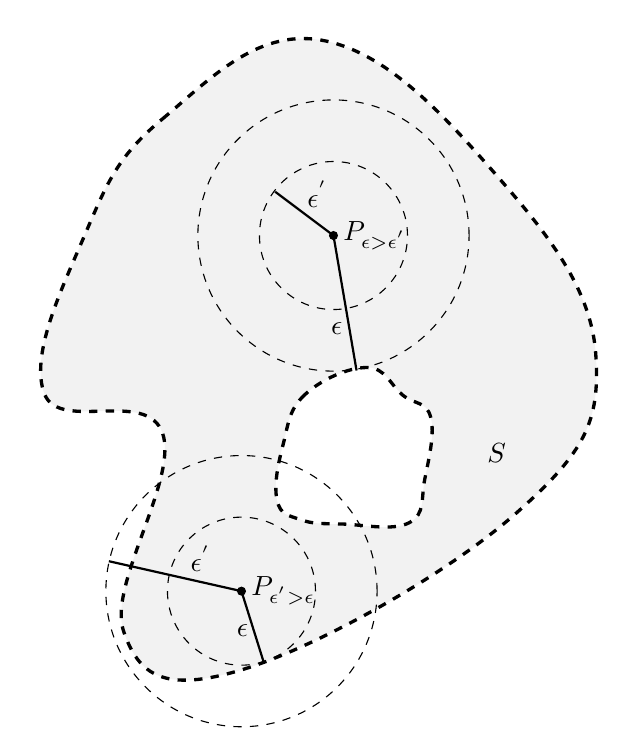
\begin{tikzpicture}

\draw [very thick,dashed,fill=gray!10] plot[smooth cycle, tension=.7] coordinates {(-4,4.5) (-3,6) (-1,7) (1.2182,5.305) (2.5,3) (1.5,1) (-2,-1) (-3.5,-0.5) (-3,2) (-4.5,2.5)};
\draw [very thick,dashed,fill=white]  plot[smooth cycle, tension=.7] coordinates {(-0.4047,2.84) (-1.1942,2.4963) (-1.4728,1.8555) (-1.5471,1.1497) (-1.2498,0.9082) (-0.7205,0.8525) (0.134,0.8711) (0.3289,1.4282) (0.4032,2.2084) (0.0503,2.487) };

\coordinate (S) at (1,2);
\node[{anchor=north west }] at (S){$S$};
\coordinate (N) at (-2,0) {};
\draw [black,dashed]  (N)circle (49pt);: 
\draw  [black,dashed](N) circle (0.94);
\draw[fill=black]  (N) circle (0.05);

\coordinate (N0) at (-1.7198,-0.8952) {} {};
\coordinate (N1) at (-3.6839,0.38) {} {} {} {};
\draw[ thick ]    plot[] coordinates { (N1)(N)  };
\draw[ thick ]    plot[] coordinates { (N0)(N)  };
\coordinate (T0) at (-2.1834,-0.7031) {} {} {} {} {};
\coordinate (T1) at (-2.2653,0.1265) {} {} {} {};
\node[{anchor=south west }] at (T0){$\epsilon$};
\node[{anchor=south east }] at (T1){$\epsilon^{'}$};
\node[right] at (N){$P_{\epsilon^{'}>\epsilon}$};


\coordinate (N2) at (-0.8317,4.5164) {} {};
\draw [black,dashed]  (N2)circle (49pt);: 
\draw  [black,dashed](N2) circle (0.94);

\coordinate (N20) at (-0.5385,2.802) {} {} {};
\coordinate (N21) at (-1.5724,5.0726) {} {} {};
\draw[ thick ]    plot[] coordinates { (N21)(N2)  };
\draw[ thick ]    plot[] coordinates { (N20)(N2)  };
\coordinate (T20) at (-0.9864,3.1348) {} {} {} {} {};
\coordinate (T21) at (-0.7827,4.7518) {} {} {};
\node[{anchor=south west }] at (T20){$\epsilon$};
\node[{anchor=south east }] at (T21){$\epsilon^{'}$};
\node[right] at (N2){$P_{\epsilon>\epsilon^{'}}$};;
\draw[fill=black]  (N2) circle (0.05);
\end{tikzpicture}\\
\caption{$\epsilon$-neighbourhood for the open non empty set $S$   }
\label{fig:fig_p8a}
\end{figure}
$i)\quad \mathbf{\epsilon^{'}>\epsilon}$\\\\
In that case we will have $N(p;\epsilon)\subset N(p;\epsilon^{'})$. This means that $N(p;\epsilon)\cap S \subset N(p;\epsilon^{'})\cap S$ and as $N(p;\epsilon)\cap S = N(p;\epsilon)\neq \emptyset$ we conclude $N(p;\epsilon^{'})\cap S\neq \emptyset$.\\\\
$ii)\quad \mathbf{\epsilon}>\epsilon^{'}$\\\\
In that case we will have $N(p;\epsilon^{'})\subset N(p;\epsilon)$. As $N(p;\epsilon)\subset S$ we also have $N(p;\epsilon^{'})\subset S$ and conclude $N(p;\epsilon^{'})\cap S\neq \emptyset$.\\\\
So, for all cases of $\epsilon^{'}$ we get the conclusion 
$$\forall p\in S, \forall\, \epsilon^{'}>0: N(p;\epsilon^{'})\cap S\neq \emptyset $$ Can we prove that also
\begin{align}
\forall p\in S, \forall\, \epsilon^{'}>0: \left(N(p;\epsilon^{'})-\{p\}\right)\cap S\neq \emptyset
\end{align}
Suppose, 
$$\forall p\in S, \forall\, \epsilon^{'}>0: \left(N(p;\epsilon^{'})-\{p\}\right)\cap S= \emptyset $$
This means that $p$ would be the only element common to $N(p;\epsilon^{'})$ and $S$. This is not possible as $\epsilon^{'}$ being greater than $0$ means that $N(p;\epsilon^{'})$ contains other elements than $p$ and as $N(p;\epsilon^{'})\subset S$ these other elements must also belong to $S$, hence $\left(N(p;\epsilon^{'})-\{p\}\right)\cap S \neq \emptyset $ and conclude that $(1)$ is a true statement and thus $p$ is a limit point of $S$. As $p$ was arbitrary chosen, this yields for all elements of $S$ and thus every point of $S$ is a limit point of $S$.  
$$\lozenge$$
Example of an open nonempty subset of $\Breal^n$ that contains all of its limit points.\\\\
$$S=\Breal^n$$
$$\blacklozenge$$\\


\subsection{}
%\subsubsection{}{}
\begin{tcolorbox}

Suppose that $\mathscr{K}$ is a collection of subsets of $\Breal^n$. Suppose $p$ is a limit point of $\bigcup \mathscr{K}$. Is $p$ necessarily a limit point of at least one $A\in \mathscr{K}$?
\end{tcolorbox}
We give a counterexample to prove this is not true.\\\
\begin{figure}[H]%
    \centering
\begin{tikzpicture} [scale=0.5,c/.style={insert path={circle[radius=1pt]}},spy using outlines={circle, magnification=20, size=2cm, connect spies}]     
    \pgfplotsset{compat=1.12};
		\tdplotsetmaincoords{0}{0};
\pgfplotsset{every axis/.append style={
		scale=1,
		axis lines=center,
		axis on top,
		xlabel={$x$},
		ylabel={$y$},
               axis x line=middle,    % put the x axis in the middle
               axis y line=middle,    % put the y axis in the middle
               %x axis line style={-latex, ultra thin}, % arrows on the axis
               y axis line style={draw opacity=1},
                x axis line style={draw opacity=1},
            }}
            
	\begin{axis}
		[ultra thin,
		xmin=-0.1,
		xmax=1.25,
		ymin=-0.75,
		ymax=0.75,
		ytick=\empty,
		xtick=\empty,
	axis equal, 
		]

	\coordinate (x0) at ({0},{0});
	\coordinate (x1) at ({1},{0});
	\coordinate (p1) at ({0.5},{0});
	
	\draw  (p1) [c];
	\node[tdplot_main_coords,{anchor=south east }] at (x0){$0$};
	\node[tdplot_main_coords,{above}] at (p1){$\frac{1}{2}$};

\draw[line width=0.01mm] (p1) circle[radius={0.25}];
\draw[line width=0.01mm] (p1) circle[radius={0.375}];
\draw[line width=0.01mm] (p1) circle[radius={0.4375}];
\draw[line width=0.01mm] (p1) circle[radius={0.46875}];
\draw[line width=0.01mm] (p1) circle[radius={0.484375}];
\draw[line width=0.01mm] (p1) circle[radius={0.4921875}];
\draw[line width=0.01mm] (p1) circle[radius={ 0.49609375}];
\draw[line width=0.01mm] (p1) circle[radius={0.498046875}];
\draw[line width=0.01mm] (p1) circle[radius={0.4990234375}];
 
\end{axis}
\spy [gray!80] on (0.65,1.42)
             in node [left] at (0.25,0);
\end{tikzpicture}\\
\caption{Open subsets $K_n=\{x:|x-(\half,0)|< \frac{2^n-1  }{2^{n+1}},\, n\in\Pee\}$ in $\Breal^2$.}
\label{fig:fig_p8a}
\end{figure}
In $\Breal^2$, take the open subsets $K_n=\{x:|x-(\half,0)|<\frac{2^n-1}{2^{n+1}},\, n\in \Pee\}$ and $\mathscr{K}=\{K_n,\,n\in \Pee \}$. This set for $\Breal^2$ is illustrated in the figure above.\\\\
$\hat{O}=(0,0)$ is a limit point for $\bigcup \mathscr{K}$. \\
Indeed, choose an arbitrary $\epsilon >0$. If $\hat{O}$ is a limit point of $\bigcup \mathscr{K}$, then we must have 
$$\forall \epsilon :\left(N(\hat{O};\epsilon)-\{\hat{O}\}\right)\cap \bigcup \mathscr{K}\neq \emptyset$$ Consider a point $(x,0)\in K_n\subset \bigcup \mathscr{K} $. We have $|x-\half|<\frac{2^n-1}{2^{n+1}}$ or 
\begin{align}
-\frac{2^n-1}{2^{n+1}}<&x-\half<\frac{2^n-1}{2^{n+1}}\\
\Leftrightarrow\quad  \frac{1}{2^{n+1}}<&x<1-\frac{1}{2^{n+1}}
\end{align}
Consider the points $(x^{'},0)\in N(\hat{O};\epsilon)$. We have $|x^{'}|<\epsilon$ or 
\begin{align*}
-\epsilon<&x^{'}<\epsilon
\end{align*}
and for $\left(N(\hat{O};\epsilon)-\{\hat{O}\}\right)$, considering only the positive $x^{'}$'s
\begin{align}
0<&x^{'}<\epsilon
\end{align}
Considering $(2)$ and $(3)$, we can always find a $n$ such that $\frac{1}{2^{n+1}}<\epsilon$. Hence  $\left(N(\hat{O};\epsilon)-\{\hat{O}\}\right)\cap K_n= \left(\frac{1}{2^{n+1}},\epsilon\right)\neq \emptyset$ and thus as $K_n\subset  \bigcup \mathscr{K}$ we have
$$\forall \epsilon :\left(N(\hat{O};\epsilon)-\{\hat{O}\}\right)\cap \bigcup \mathscr{K}\neq \emptyset$$.\\\\
On the other hand, for a given $K_n\in \mathscr{K}$ it is clear that $\hat{O}$ is not a limit point as we can always find an $\epsilon < \frac{1}{2^{n+1}}$, meaning that $K_n$ and $\left(N(\hat{O};\epsilon)-\{\hat{O}\}\right)$ have no common points, hence, $\hat{O}$ is not a limit point of $K_n$.
$$\blacklozenge$$\\


\subsection{}
%\subsubsection{}{}
\begin{tcolorbox}
If your answer to Exercise $5$ is no, prove the following: Suppose that $\mathscr{K}$ is a finite collection of subsets of $\Breal^n$. If $p$ is a limit point of $\bigcup \mathscr{K}$ , then $p$ is a limit point of at least one $A \in \mathscr{K}$.
\end{tcolorbox}
Be $p$ a limit point of $\bigcup \mathscr{K}$. This means
$$\forall  \epsilon >0, \left(N(p;\epsilon)-\{p\}\right)\cap \bigcup \mathscr{K}\neq \emptyset$$

Be $S=\left(N(p;\epsilon)-\{p\}\right)\cap \bigcup \mathscr{K}\neq \emptyset$. This means $\exists x\in\Breal^n$ such that $ x\in S\Et x\in \bigcup\mathscr{K}$, the latter means that $x$ must be an element of at least one $A^{*}\in \mathscr{K}$.\\
But $x$ must also be an element of $\left(N(p;\epsilon)-\{p\}\right)$ so we have 
$$\forall  \epsilon >0, \left(N(p;\epsilon)-\{p\}\right)\cap A^{*}\neq \emptyset$$
Hence, there exists at least one $A^*$ for which $p$ is a limit point.
$$\blacklozenge$$\\

\subsection{}
%\subsubsection{}{}
\begin{tcolorbox}
Let $S\subset \Breal^n$  and let $z$ be a limit point of $S$. Show that for every $\epsilon > 0$ , $N(z; \epsilon)\cap S$ is an infinite set.
\end{tcolorbox}
We have 
\begin{align}
&\forall  \epsilon >0, \left(N(z;\epsilon)-\{z\}\right)\cap S\neq \emptyset\\
\implies \quad &\forall  \epsilon >0, N(z;\epsilon)\cap S\neq \emptyset
\end{align}
Suppose $K=N(z;\epsilon)\cap S$ is a finite set. Be $K=\{x_1,\, x_2,\, \dots ,\, x_N\}$ and $E=\{|x_1-z|,\, |x_2-z|,\, \dots ,\, |x_N-z|\}$. Put $\delta = \min{E}$. Then for any $\epsilon^{'}<\delta $ we have 
\begin{align}
N(z;\epsilon^{'})\cap S=\emptyset\quad , \epsilon^{'}<\delta 
\end{align}
We get a contradiction as $(3)$ puts a constraint on the requirement ($\forall$) in  $(2)$  and thus we conclude \\
$$N(z;\epsilon^{'})\cap S\text{ is a infinite set.}$$
$$\blacklozenge$$\\


\mysection{39}{Closed subsets of $\Breal^n$}
\subsection*{Clarifications on Theorem 39.5}
\textit{For each subset of $\Breal^n$, $cl (S)$ is a closed subset of $\Breal^n$.}\\
(Each step in the book is labelled, so we can refer to it in the following steps).\\\\
Proof. \\
(a) Let $x$ be a limit point of $cl (S)$. \\
(b) We wish to show that $x \in \, cl (S)$.\\
(c) If $x \not \in \, cl (S)$, then $x \not \in \, S$ and $x$ is not a limit point of $S$.\\
    \textit{$\bullet\quad$(This is because $cl(S)$ by definition must contain all limit point of $S$).}\\
(d) Hence, there is an $\epsilon  > 0$
such that $N(x; \epsilon)\subset \Breal^n- S$. \\
\textit{$\bullet\quad$(This is by the definition of a limit point i.e. $\forall\epsilon>0, (N(x; \epsilon)-\{x\})\cap S\neq \emptyset$. As $x$ is not a limit point of $S$ (see (b)) $(N(x; \epsilon)-\{x\})\cap S= \emptyset$ and thus all elements of $N(x; \epsilon)$ must be an element of the complement of $S$ i.e. $\Breal^n-S$).}\\
(e) However, since $x$ is a limit point of $cl (S)$, there is a
point $z \in \,  cl (S)$ such that $0 < d(x, z) < \epsilon$.\\
\textit{$\bullet\quad$(This follows from the definition of a limit point $\forall\epsilon>0, (N(x; \epsilon)-\{x\})\cap S\neq \emptyset$ and thus there must be at least one $z\in(N(x; \epsilon)-\{x\})\cap S$ ).}\\
(f) Then since $z\not\in S$, $z$ is a limit point of $S$.\\
\textit{$\bullet\quad$(This is because $cl(S)$ by definition must contain all limit point of $S$).}\\
(g) Since $\epsilon - d(x, z) > 0$ and $z$ is a limit point of $S$, there is a point $y\in S$ such that
$d(y, z) \leq  \epsilon - d(x, z)$.\\
(h) However, $d(x, y) \leq d(y, z) + d(z, x) < \epsilon - d(x, z) +d(z, x) = \epsilon$ (see accompanying figure).\\
(i) Hence, $y\in S\cap N(x;\epsilon)$, contrary to the way in which $\epsilon$ was chosen.
\\
\textit{$\bullet\quad$(This follows from (d) $N(x; \epsilon)\subset \Breal^n- S)$}, meaning that $S$ and $N(x; \epsilon$ can't have common elements)\\
\newpage

\renewcommand{\thesubsection}{\thesection.\arabic{subsection}}
\setcounter{subsection}{0}

\subsection{}
%\subsubsection{}{}
\begin{tcolorbox}
Suppose that $F$ is a finite subset of $\Breal^n$. Is $F$ necessarily closed in $\Breal^n$?
\end{tcolorbox}
Consider $\sim F$. Then, all $p\in F$ are limit points of $\sim F$. Indeed, we have, $\forall \epsilon>0: \left(N(p;\epsilon)-\{p\}\right)\subset \sim F$ and thus $\forall \epsilon>0: \left(N(p;\epsilon)-\{p\}\right)\cap \sim F\neq \emptyset$. Conclusion $p$ is a limit point of $\sim F$. and as $p\not\in \sim F$ we can rewrite this as $\forall \epsilon>0: N(p;\epsilon)\cap \sim F\neq \emptyset$. Also, consider an arbitrary point $z\in\sim F$. Be $E=\{|p_1-z|,|p_2-z|,,\dots, |p_n-z|\}$ where the $p_i$ are the element of $F$. Be $\delta = \min E$ and choose $\epsilon^{'} < \delta$, the we will have that $N(z;\epsilon^{'})\subset \sim F$ and thus $\sim F$ is an open subset and by theorem $\mathbf{39.2}$ $F$ is a closed subset.
$$\blacklozenge$$\\


\subsection{}
%\subsubsection{}{}
\begin{tcolorbox}
Prove Theorems $\mathbf{39.2}\Et \mathbf{39.3}$.
\end{tcolorbox}
$$ $$
$\mathbf{39.2}$ Let $S\subset \Breal^n$. Then $S$ is closed if and only if its complement is open in $\Breal^n$.
$$\implies$$
\textbf{$\mathbf{S}$ is closed.}\\
Be $p\in \, \sim S$. Then, $p\not \in  S$ and thus $p$ can not be a limit point of $S$. Hence, the statement $\forall \epsilon >0,\left(N(p;\epsilon)-\{p\}\right)\cap S\neq \emptyset$ is false. We have,
\begin{align*}
&\neg\left(\forall \epsilon >0,\left(N(p;\epsilon)-\{p\}\right)\cap S\neq \emptyset\right)\\
\Leftrightarrow\quad &\exists\, \epsilon >0,\left(N(p;\epsilon)-\{p\}\right)\cap S= \emptyset\\
\Leftrightarrow\quad &\exists\, \epsilon >0,N(p;\epsilon)\cap S= \emptyset
\end{align*}
The last statement follows from the fact that $p\not\in S$, hence the presence of $p$ in $N(p;\epsilon)$ is of no object for the statement.
By the last statement , $N(p;\epsilon)\not\subset S$ and thus $N(p;\epsilon)$ lies completely in the complement of $S$ and we get for any arbitrary $p\in(\sim S)$:
$$\exists\, \epsilon >0,N(p;\epsilon)\subset (\sim S)$$
proving that $\sim S$ is an open set.
$$\lozenge$$\\\\
$$\Leftarrow$$
\textbf{$\mathbf{\sim S}$ is open.}\\
Be $q$ a limit point of $S$ but not in $S$, then $q\in(\sim S)$. As $\sim S$ is an open set we have $\exists\,\epsilon >0, N(q;\epsilon)\subset (\sim S)$ and thus $\exists\,\epsilon >0, N(q;\epsilon)\not \subset S$ giving $\exists\,\epsilon >0, N(q;\epsilon) \cap S=\emptyset$. The presence of $q$ in $N(q;\epsilon)$ does not change the last statement and we have
$$\exists\,\epsilon >0, \left(N(q;\epsilon)-\{q\}\right)\cap S=\emptyset$$
We have a contradiction as we supposed that $q$ was a limit point of $S$, hence the supposition that $q$ is not in $S$ is wrong. So a limit point of $S$ must be in $S$ and thus $S$ is closed.
$$\lozenge$$
$\mathbf{39.3}$\\ 
$\mathbf{(a)}$ \textbf{The empty set and $\Breal^n$ are closed subsets of $\Breal^n$.\\\\}
We use in both case theorem $\mathbf{39.2}$ \textit{(Let $S \subset \Breal^n$. Then $S$ is closed if and only if its complement
is open in $\Breal^n$)}.\\\\
$\bullet$ As $\emptyset=\sim \Breal^n$ and from $\mathbf{37.2}$ we know that  $\Breal^n$ is an open set. By theorem $\mathbf{39.2}$ we then know that it's complement is closed. Hence, $\emptyset$ is closed. \\\\
$\bullet$ As $\Breal^n =\sim \emptyset $ and from $\mathbf{37.2}$ we know that  $\emptyset$ is an open set. By theorem $\mathbf{39.2}$ we then know that it's complement is closed. Hence, $\Breal^n$ is closed. 
$$\lozenge$$
For the following statements we use the De Morgan's laws
\begin{align}
\bigcup\{\sim K:K\in\mathscr{K}\} = \sim \left(\bigcap\{ K:K\in\mathscr{K}\}\right)\\
\bigcap\{\sim K:K\in\mathscr{K}\} = \sim \left(\bigcup\{ K:K\in\mathscr{K}\}\right)
\end{align}
 and also the results of exercise $\mathbf{2.37.2}$
 \begin{align}
 \textit{The union of an arbitray colection of open subsets of }\Breal^n\textit{ is open.}\\
 \textit{The intersection  of a finite colection of open subsets of }\Breal^n\textit{ is open.}
 \end{align}
$\mathbf{(b)}$ \textbf{The intersection of an arbitrary nonempty collection of closed sets is closed}\\\\
We know that $K$ is closed and thus $\sim K$ is open. By $(3)$ we have
\begin{align*}
& \bigcup\{\sim K:K\in\mathscr{K}\} \text{ is open}\\
\text{and by (1) }\quad  & \bigcup\{\sim K:K\in\mathscr{K}\} = \sim \left(\bigcap\{ K:K\in\mathscr{K}\}\right)\\
\implies\quad &   \sim\left(\bigcap\{ K:K\in\mathscr{K}\}\right) \text{ is open}\\
\end{align*}
By theorem $\mathbf{39.2}$ we conclude 
$$\bigcap\{ K:K\in\mathscr{K}\} \text{ is closed.}$$\\\\
$\mathbf{(c)}$ \textbf{The union of a finite collection of closed sets is closed.}\\\\
We know that $K$ is closed and thus $\sim K$ is open. By $(4)$ we have (as $\mathscr{K}$ is finite)
\begin{align*}
& \bigcap\{\sim K:K\in\mathscr{K}\} \text{ is open}\\
\text{and by (2) }\quad  & \bigcap\{\sim K:K\in\mathscr{K}\} = \sim \left(\bigcup\{ K:K\in\mathscr{K}\}\right)\\
\implies\quad &   \sim\left(\bigcup\{ K:K\in\mathscr{K}\}\right) \text{ is open}
\end{align*}
By theorem $\mathbf{39.2}$ we conclude 
$$\bigcup\{ K:K\in\mathscr{K}\} \text{ is closed.}$$


$$\blacklozenge$$\\


\subsection{}
%\subsubsection{}{}
\begin{tcolorbox}
Is the set in Example $\mathbf{37.3 }$ a closed set?
\end{tcolorbox}
Consider $S=\Breal\times\{0\}$. Then, $\sim S=\emptyset\times \Breal_{0}$. We know that $\emptyset$ is open. Also $\Breal_{0}$ is open (choose for any $p\in \Breal_{0}$ an $\epsilon<\frac{|p|}{2}$, giving $N(p;\epsilon)\subset \Breal_{0}$.)\\
So $\sim S$ is open and by theorem $\mathbf{39.2}$ we conclude that $S$ is a closed subset of $\Breal^2$.
$$\blacklozenge$$\\


\subsection{}
%\subsubsection{}{}
\begin{tcolorbox}
Let $a \Et b$ be real numbers and let $S$ be the following subset of $\Breal^2$. $ S = \{(x,y):ax + by \leq 1\}$. Is $S$ a closed set?
\end{tcolorbox}
$ \sim S = \{(x,y):ax + by > 1\}$ is open and by by theorem $\mathbf{39.2}$ we conclude that $S$ is a closed subset of $\Breal^2$.
$$\blacklozenge$$\\

\subsection{}
%\subsubsection{}{}
\begin{tcolorbox}
Let $S$ be a subset of $\Breal^n$. Let $S^{'}= \{x:x \in \Breal^n \Et x \text{ is a limit point of } S\}$. Is $S^{'}$ necessarily a closed set?
\end{tcolorbox}
The proof is analog to the proof of Theorem $\mathbf{39.5}$.\\
Let $x$ be a limit point of $S^{'}$. We wish to show that $x \in \, S^{'}$.\\
If $x \not \in \, S^{'}$, then  $x$ is not a limit point of $S$
    \textit{(This is because $S^{'}$, by definition, must contain all limit point of $S$).}\\
Hence, there is an $\epsilon  > 0$
such that $N(x; \epsilon)\subset \Breal^n- S$ 
\textit{(This is by the definition of a limit point i.e. $\forall\epsilon>0, (N(x; \epsilon)-\{x\})\cap S\neq \emptyset$. As $x$ is not a limit point of $S$ , there exists an $\epsilon$ such that  $(N(x; \epsilon)-\{x\})\cap S= \emptyset$ and thus all elements of $N(x; \epsilon)$ must be an element of the complement of $S$ i.e. $\Breal^n-S$).}\\
However, since $x$ is a limit point of $S^{'}$, there is a
point $z \in \,  S^{'}$ such that $0 < d(x, z) < \epsilon$ 
\textit{( This follows from the definition of a limit point $\forall\epsilon>0, (N(x; \epsilon)-\{x\})\cap S\neq \emptyset$ and thus there must be at least one $z\in(N(x; \epsilon)-\{x\})\cap S$ ).}\\
Then since $z\in S^{'}$, $z$ is a limit point of $S$ 
\textit{(This is because $S^{'}$ by definition must contain all limit point of $S$).}\\
Since $\epsilon - d(x, z) > 0$ and $z$ is a limit point of $S$, there is a point $y\in S$ such that
$d(y, z) \leq  \epsilon - d(x, z)$.\\
However, $d(x, y) \leq d(y, z) + d(z, x) < \epsilon - d(x, z) +d(z, x) = \epsilon$.\\
Hence, $y\in S\cap N(x;\epsilon)$, and we get a contradiction as $N(x; \epsilon)\subset \Breal^n- S$, meaning that $S$ and $N(x; \epsilon)$ can't have common elements.\\
Conclusion $x$ must be an element of $S^{'}$. So, $S^{'}$ is a closed subset of $\Breal^n$.
$$\blacklozenge$$\\

\subsection{}
%\subsubsection{}{}
\begin{tcolorbox}
Give an example of a countable collection $\mathscr{K           }$ of closed subsets of $\Breal^2$ such that $\bigcup\mathscr{K}$ is not closed.
\end{tcolorbox}
See Exercise $\mathbf{2.38.2}$ where the subset $\{\hat{O}\}= \{(0,0)\}$ is a limit point of $\mathscr{K}$ but no element of it.
$$\blacklozenge$$\\

\subsection{}
%\subsubsection{}{}
\begin{tcolorbox}
Let $S$ be a subset of $\Breal^n$. Let $F$ consist of all points $p$ in $\Breal^n$ such that for each $\epsilon > 0, \, N(p; \epsilon)\cap S \neq \emptyset$ and $N(p;\epsilon)\cap \left(
\sim S\right)  \neq \emptyset$. Is $F$ necessarily a closed set?
\end{tcolorbox}
Consider $S=\{p\}$ a set in $\Breal^n$ consisting of a single point. Then, $\forall \epsilon > 0, \, N(p; \epsilon)\cap S = \{p\}(\neq \emptyset)$, which implies that $p\in F$. Also, $N(p;\epsilon)\cap \left(\sim S\right)\neq \emptyset$ as $N(p;\epsilon)-\{p\}$ contains only elements of $\sim S$. Also, no other element $q$ of $\sim S$ can comply with the condition $\forall \epsilon > 0, \, N(q; \epsilon)\cap S \neq \emptyset$ and hence $F=S$. So $F$ has no limit point (and thus does not contain any), hence $F$ is not closed.

$$\blacklozenge$$\\

\subsection{}
%\subsubsection{}{}
\begin{tcolorbox}
Show that lines and polygons are closed subsets of $\Breal^n$ (see $\mathbf{35.5}\Et \mathbf{ 35.6}$).
\end{tcolorbox}

First note that, for polygons, by theorem $\mathbf{39.3 (c)}$ (\textit{The
union of a finite collection of closed sets is closed}) it suffice to prove that a line is a closed subset as a polygon is the union of a finite number of line segments and the union of a finite collection of closed sets is closed.\\
Recall the definition of a line segment $L(a,b)$ determined by $a \Et b$:\\
$$L=\{x:x=(1-t)a+tb,\, t\in \Breal_{[0,1]}\}$$
Be a $p$ a limit point of the line $L(a,b)$. Then, $\forall \epsilon: \left( N(p;\epsilon)-\{p\}\right)\cap L(a,b)\neq \emptyset$. This means that $\exists x\in L(a,b)$ which is also an element of $N(p;\epsilon)$. This implies 
$$ d(p;x)<\epsilon$$
Suppose that $p\not\in L(a,b)$. This implies
$$\not\exists\, t\in\Breal : p= (1-t)a+bt$$
Consider the set $$D=\{d=d(p;x):x= (1-t)a+bt,\forall t\in\Breal \}$$
As $p\not\in L(a,b)$, the ordered set $(D,\leq)\subset (\Breal,\leq)$ does not contain the element $d=0$, hence $D$ has a lower bound $=0\not \in D$.\
By the least upper bound axiom on page $\mathbf{61}$ and it's corollary (exercise $2$ page $62$) $D$ has a greatest lower bound. Be $g.l.b\,  D=\delta$. We have 
$$0<\delta$$ and thus 
$$\forall\epsilon >0: 0<\delta \leq d(p;x)<\epsilon$$
But this inequality must be true for any $\epsilon>0$. We get a contradiction as this inequality can't be satisfied for $0<\epsilon <\delta$ and thus our assumption the $p\not\in L(a,b)$ is false.


$$\blacklozenge$$\\
\newpage

\mysection{40}{Bounded subsets of $\Breal^n$}
\subsection*{Remark on 40.4 -  The Bolzano-Weierstrass Theorem}
\begin{figure}[H]%
    \centering
\begin{tikzpicture}
\coordinate (O) at (0,0);
\coordinate (X1) at (7,0) {};
\coordinate (X2) at (0,7) {};
\node[right] at (X1){\tiny$X_1$};
\node[above] at (X2){\tiny$X_2$};
\draw[ thick ]   (O)--(X1) ;
\draw[ thick ]  (O)--(X2);
\fill[thick,pattern=north west lines, pattern color=gray!50] (0.8,5.6)rectangle (4.8,1.6);
\coordinate (S) at (2,5.2) {} {};
\fill[fill=white](S) circle (0.2);
\node[] at (S){\tiny$S$};

\draw[](0.8,5.6) node (v2) {} rectangle (4.8,1.6) node (v4) {};
\coordinate (K0) at (1.2,2) {} {} {} {};
\node[right] at (K0){\tiny$K_0$};
\node[below] (v5) at (0.8,0) {\tiny$\alpha$};
\node[below] (v6) at (4.8,0) {\tiny$\beta$};
\node[left] (v3) at (0,1.6) {\tiny$\alpha$};
\node[left] (v1) at (0,5.6) {\tiny$\beta$};
\draw[dashed]  (v1) -- (v2);
\draw[dashed]   (v3) -- (v4);
\draw [dashed]  (v2) -- (v5);
\draw[dashed]   (v4) -- (v6);
\coordinate (v8) at (4.8,3.6) {};
\coordinate (v7) at (0,3.6) {};
\coordinate (v9) at (2.8,5.6) {};
\coordinate (v10) at (2.8,0) {};
\draw[dotted,very thick]  (v7) -- (v8);
\draw[dotted,very thick]   (v9) -- (v10);
\coordinate (j1) at (3.8,3) {} {} {};
\coordinate (j2) at (2.2,4.8) {} {} {};
\node[below] at (j1) {\tiny$J1$};
\node[below] at (j2) {\tiny$J2$};
\draw [thick,decorate,
	decoration = {brace,raise=5pt}] (2.8,3.6) --  (2.8,5.6);
\draw [thick,decorate,
	decoration = {brace,raise=5pt}] (4.8,3.6) --  (2.8,3.6);
	
	\draw [thick,decorate,
	decoration = {brace,raise=5pt}] (4.8,-0.2) --  (2.8,-0.2);
	
	\draw [thick,decorate,
	decoration = {brace,raise=5pt}] (-0.6,3.6) --  (-0.6,5.6);
\fill[thick,pattern=north east lines, pattern color=gray!50] (2.8,5.6) rectangle (4.8,3.6);

\coordinate (L1) at (6.2,2.6) {} {} {} {} {};
\node[below]at (L1){\tiny$K_1=J_1\times J_2$};
\node (v11) at (4.6,4.2) {};
\draw[-{Latex[length=2mm]}]  plot[smooth, tension=.7] coordinates {(L1) (5.6,3) (5.4,3.6) (v11)};
\draw [thick,decorate,
	decoration = {brace,raise=5pt}] (2.8,5.6) --  (3.8,5.6);
\draw [thick,decorate,
	decoration = {brace,raise=5pt}] (4.8,5.6) --  (4.8,4.6);

\coordinate (pj1)at (2.8,4.6) {};
\coordinate (pj2) at (4.8,4.6) {};
\coordinate (pj3)at (3.8,5.6) {};
\coordinate (pj4) at (3.8,3.6) {};

\draw[dotted,very thick]  (pj1) -- (pj2);
\draw[dotted,very thick]   (pj3) -- (pj4);
\coordinate (lab1) at (3.4,6) {};
\coordinate (lab2) at (5.2,5.1) {};
\node[above] at (lab1) {\tiny$\frac{\beta-\alpha}{2^2}$};
\node[right] at (lab2) {\tiny$\frac{\beta-\alpha}{2^2}$};
\fill[very thick,pattern=dots, pattern color=gray!90] (2.8,5.6) rectangle (3.8,4.6);
\coordinate (L2) at (4.8,6.2) {} {} {} {} {} {};
\node[above]at (L2){\tiny$K_2$};
\node (v15) at (3.6,5) {};
\draw[-{Latex[length=2mm]}]  plot[smooth, tension=.7] coordinates {(L2) (4.4,6) (4.2,5.2) (v15)};

\node at (-1.2,4.6) {\tiny$\frac{\beta-\alpha}{2}$};;
\node at (3.8,-0.8) {\tiny$\frac{\beta-\alpha}{2}$};
\draw[thick,dashed,gray!80]  plot[smooth cycle, tension=.7] coordinates { (4.2551,4.3997) (4.3578,3.9183) (4.1525,2.6636)   (3.1345,1.7953) (2.227,1.6929)   (1.8087,2.1584) (2.3138,2.8529) (2.0849,3.8078)   (1.501,5.2836) (2.1481,5.5678) (2.6294,5.473) (3.0319,5.3468) (3.2608,5.2047)};
\end{tikzpicture}\\
\caption{The Bolzano-Weierstrass Theorem}
\label{fig:fig_p8a}
\end{figure}
The succcesive partition of the close interval $K^{(p)}_i$ in equal $n^2$ closed intervals $K^{(q)}_{i+1}(q=1,2,\dots 2^n)$  makes that we can always choose one of this intervals such that $S\cap K^{(q^{'})}_{i+1}\neq \emptyset$
\newpage
\renewcommand{\thesubsection}{\thesection.\arabic{subsection}}
\setcounter{subsection}{0}



\mysection{41}{ Convergent sequences in $\Breal^n$}

\subsection*{Remark on 41.3 on the "boundness" of a convergent sequence}
\begin{figure}[H]%
    \centering
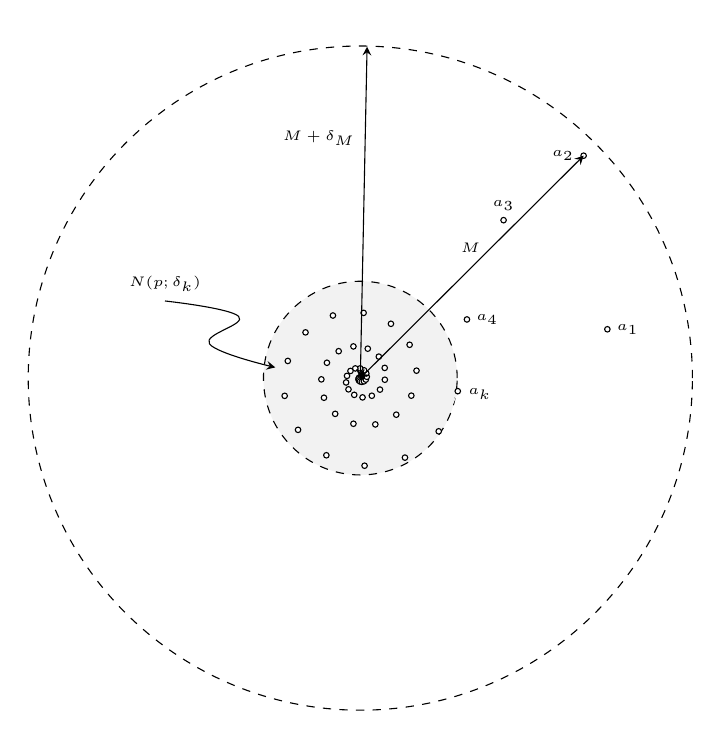
\begin{tikzpicture}
   \coordinate (O) at (0,0) {} {} {};
   \draw[dashed,fill=gray!10]  (O) circle (35pt);
\draw [gray!10,domain=0:25,variable=\t,smooth,samples=55]    plot[mark=*,mark size=1pt,,mark options={black,fill=white}] ({\t r}: {0.002*\t*\t});
   \coordinate (a3) at (1.3542,0.7447) {};
      \coordinate (a2) at (1.8193,2.0056) {} {} {} {} {};
  \coordinate (a1) at (2.836,2.8246) {} {};
   \coordinate (a0) at (3.1376,0.62) {} {} {};
\draw [white] plot[white,mark=*,mark size=1pt,,mark options={black,fill=white},smooth, tension=.7] coordinates {(a0) (a1) (a2) (a3)};

      \coordinate (O) at (0,0) {} {} {};
   \draw[dashed]  (O) circle (120pt);
   \node[right] at (a0) {\tiny$a_1$};
   \node[left]  at (a1) {\tiny$a_2$};
   \node[above]  at (a2) {\tiny$a_3$};
   \node[right]  at (a3) {\tiny$a_4$};
   \coordinate (ak) at (1.25,-0.2) {} {} {};
     \node[right]  at (ak) {\tiny$a_k$};
\node (v1) at (0.0885,4.3332) {};
\draw[<->,>=stealth]  (O)--(a1);
\node at (1.4005,1.6608) {\tiny$M$};
\draw[<->,>=stealth]  (O)--(v1);
\node[left] at (0.0577,3.0487) {\tiny$M+\delta_M$};
\draw[->,>=stealth]  plot[smooth, tension=.7] coordinates {(-2.4807,0.9793) (-1.5451,0.784) (-1.9152,0.4344) (-1.08,0.136)};
\node[above] at (-2.4807,0.9793) {\tiny$N(p;\delta_k)$};
\end{tikzpicture}\\
\caption{Example in $\Breal^2$ of a convergent and hence, bounded sequence}
\label{fig:fig_p8a}
\end{figure}
In the book, an $\epsilon=1$ is taken to prove that a convergent sequence is bounded. But any positive number can be chosen to prove the boundness as seen in the figure $2.6$.\\
The sequence begins with $a_1$ and we choose an arbitrary $\delta_k$. As the sequence is convergent this means that for this $\epsilon= \delta_k$ there must be a positive integer $k$ such that $d(L;a_i)<\delta_k$ for all $i>k+1$. And, if we take as $M=max \{d(a_i,L):i\in \Pee\}$ then $\forall i\in \Pee, \forall \delta_M>0: d(a_i,L)< M+\delta_m$
\renewcommand{\thesubsection}{\thesection.\arabic{subsection}}
\setcounter{subsection}{0}
\\\\
\subsection*{Remark on Theorem 41.4 on the convergence of a subsequence of a bounded sequence}

Proof.
 \textit{Suppose the range of $(a_i)$ is a finite set. Then there is a strictly increasing sequence of positive integers $(n_i)$ and a point $z \in\Breal^n$ such that $a_{n_i}=z$ for 
$i\in\Pee$. Hence, $\lim (a_{n_i} ) =z$ and we are through.}
\\
As an example take the sequence in $\Breal^2$ defined by
$$a_i=\left(\sin{\left(\frac{2\pi}{T}i\right)},\cos{\left(\frac{2\pi}{T}i\right)}\right)\text{ with } T\in \Pee, i\in \Pee$$
Then the range of the (bounded) sequence is finite with $T$ possible values. Define the subsequence by defining the map 
$$n_i= T(i-1)+T^{'}\text{ with } T^{'}\in\Pee \Et T^{'}\leq T$$  will map $a_{n_i}$ on one of the $T$ values and we have a convergent sequence with $a_{n_i}= C^t\quad \forall n_i$.
$$\lozenge$$\\
\textit{Next suppose the range $S$ of
$(a_i)$ is an infinite set. By the Bolzano-Weierstrass theorem there is a point $z$ that is a limit point of $S$. (We shall find a subsequence $(a_{n_i})$ of $(a_i)$ by choosing for each
$i\in \Pee$, an $(a_{n_i})$such that $d(a_{n_i} , z) < \frac{1}{i}$. However, we must be careful to choose these in such a way that $(n_i)$ is a strictly increasing sequence of positive integers. We shall do this inductively.) \\\\
Since $z$ is a limit point of $S$, there is a positive integer such that}
$$0 < d(a_{n_1}, z) < 1$$
\textit{Assume that for $1,2,\dots, h$, increasing integers ${n_1},{n_2},\dots,{n_h}$ have been chosen
such that}
$$0 < d(a_{n_i}, z) < \frac{1}{i}$$
\textbf{\textit{Since $S\cap N\left(z;\frac{1}{i+1}\right)$ is an infinite set (see Exercise 7, page 71 ), there is an integer $n_{h+1}$ such that $n_{h} < n_{h+1}$ and for which $d(a_{n_{h+1}}, z) < \frac{1}{h+1}$.} }
\begin{mdframed}
Is it so obvious that there is an integer $n_{h+1}$ such that $n_{h} < n_{h+1}$ and for which $d(a_{n_{h+1}}, z) < \frac{1}{h+1}$?\\
By assumption we have a set $K=\{a_{n_1},a_{n_2},\dots,a_{n_h}\}$ such that $0 < d(a_{n_i}, z) < \frac{1}{i}$. As $U= S\cap N\left(z;\frac{1}{i+1}\right)$ is an infinite set $U-K$ still will be an infinite set because $K$ is a finite set.\\
So, is it possible that for all elements $a_{n_p}\in U-K$ we have $n_p<n_h$? The answer is definitely negative, as the number of 'available slots' in the set $\{1,2,\dots,n_h\}$ is finite. Hence after excluding all $n_j$ such that $n_j<n_h$ we will still be able to find an infinite number of $n_k > n_h: k\geq h+1$ for which $d(a_{n_{k}}, z) < \frac{1}{k}:\quad n_k > n_h$
\end{mdframed}
\textit{Hence, by induction (see $18.4$), a strictly increasing sequence of integers $n_{i}$ has been chosen
such that $d(a_{n_{i}}, z) < \frac{1}{i}$. It is clear from the way in which the integers $(n_i)$ were
chosen that $(a_{n_i} )$ is a subsequence of $(a_{i} )$ and that $\lim (a_{n_i}) = z$.}
\newpage
\renewcommand{\thesubsection}{\thesection.\arabic{subsection}}
\setcounter{subsection}{0}

\subsection{}
%\subsubsection{}{}
\begin{tcolorbox}
Prove that if $S$ is a subset of $\Breal^n$ and $z \in \Breal^n$, then $z$ is a limit point of $S$ if and only if there exists a sequence $(a_i)$ in $S$ that converges to $z$ and which is such that $a_i\neq a_j$ for $i\neq j$.
\end{tcolorbox}
We have to prove
$$\forall \epsilon >0: \left(N(z;\epsilon)-\{z\}\right)\cap S\neq\emptyset\quad \iff\quad \exists \quad(a_i)\text{ in } S: a_i\neq a_j \text{ for } i\neq j \Et \lim a_i= z$$\\\\
$$\lozenge$$\\
$$\mathbf{\mathlarger{\implies}}$$
We have that $z$ is a limit point. So, 
\begin{align}
\forall \epsilon >0: \left(N(z;\epsilon)-\{z\}\right)\cap S\neq\emptyset
\end{align}
Let's put $\epsilon =1$ and denote 
$$D_1=\left(N(z;1)-\{z\}\right)\cap S$$
Then we can write $D_1$ as
 \begin{align}
 D_1=\{ x\in S: d(x,z)<1\}
 \end{align}
 We know that $D_1$ is an infinite set (see Exercise 7, page 71 ).\\
 Let's define 
 \begin{align}
 \mathscr{D}_1=\{d(x,z): x\in D_1\}
 \end{align}
 Obviously $\mathscr{D}_1\subset \Breal$ and is (upper) bounded and is a linearly ordered subset of $\Breal$. Using Zorn's Lemmma (page 47) we know that $\mathscr{D}_1$ has a maximal element in $\mathscr{D}_1$. Let's choose the element $a_1$ of $D_1$ for which $d(a_1,z)=\max \mathscr{D}_1$ ($a_1$ is unique as $S$, being a set, will contain only one element of the same object).\\
 Consider now 
 \begin{align}
 D_2=\{ x\in S: 0<d(x,z)<\frac{1}{2}\}-\{a_1\}
 \end{align}
 $D_2$ is still infinite. Let's repeat the procedure initiated in $(3)$ by defining $ \mathscr{D}_2=\{d(x,z): x\in D_2\}$ etc.. and choose an element $a_2$ such that $d(a_2,z)=\max \mathscr{D}_2$.\\
 Repeating this procedure gives us a sequence
  \begin{align}
 \{(1,a_1), (2,a_2),\dots, (i,a_i),\dots\}\text{ such that }0< d(a_i,z)<\frac{1}{i}\text{ for } i\in \Pee 
 \end{align}
The definition of convergence of a sequence $(a_i)$ to $z$  is:
$$\forall\epsilon > 0, \exists N\in\Pee:\, d(a_k,z) <\epsilon \text{ whenever } k \geq N $$
If we choose an arbitrary $\epsilon>0$ it suffice in $(5)$ to put $\frac{1}{i}\leq \epsilon$ or $i\geq \frac{1}{\epsilon}$ to see that the sequence in $(5)$ converges to $z$.\\\\
Finally, by the way we constructed  the sequence by defining the different subsets $D_k$ as $$D_k=\{ x\in S: 0<d(x,z)<\frac{1}{k}\}-\{a_1,\dots,a_{k-1}\}  $$ we are assured that $a_i\neq a_j$ for $i\neq j$.
$$\lozenge$$\\
$$\mathbf{\mathlarger{\Leftarrow}}$$
We know that for the sequence $(a_i)$ we have 
\begin{align}
\lim a_i= z\quad\Et a_i\neq a_j \text{ for } i\neq j
\end{align}
this implies
\begin{align}
\forall\epsilon > 0, \exists N\in\Pee:\, d(a_k,z) <\epsilon \text{ whenever } k \geq N
\end{align}
The requirement $a_i\neq a_j \text{ for } i\neq j$ in $(6)$ makes that if $z$ occurs in the sequence, it can only occur once. Be $M$ the position in the sequence were $z$ occurs, then the subsequence $(a_k):k> M$ will still converges to $z$ (construct the subsequence $(i,a_i): i>M$ and replace $N$ in $(7)$ by $N-M$).\\
So, $(7)$ can be replaced by 
\begin{align}
\forall\epsilon > 0, \exists N\in\Pee:\, 0< d(a_k,z) <\epsilon \text{ whenever } k \geq N
\end{align}
which is equivalent to state as 
$\forall \epsilon >0: \left(N(z;\epsilon)-\{z\}\right)\cap S\neq\emptyset$
$$\blacklozenge$$\\


\subsection{}
%\subsubsection{}{}
\begin{tcolorbox}
 Suppose $(a_i)$ is a sequence in $\Breal^n$ that has the following property:
For each $\epsilon > 0$, there is an integer $N$ such that $d(a_m, a_n) < \epsilon$
for $m\geq N $ and $n\geq N$. Show that $(a_i$) is a bounded sequence.
\end{tcolorbox}

$$\blacklozenge$$\\


\subsection{}
%\subsubsection{}{}
\begin{tcolorbox}
Prove that if $(a_i)$ is a convergent sequence in $\Breal^n$, then for each
subsequence $(a_{N_i})$ of $(a_i)$, $\lim (a_i) = \lim (a_{N_i})$.
\end{tcolorbox}

$$\blacklozenge$$\\

\newpage


\subsection{}
%\subsubsection{}{}
\begin{tcolorbox}
Give the details of the proof of $\mathbf{41.2}$.
\end{tcolorbox}

$$\blacklozenge$$\\


\subsection{}
%\subsubsection{}{}
\begin{tcolorbox}
Prove that a subset $S$ of $\Breal^n$ is closed and bounded if and only if
every sequence in $S$ has a convergent subsequence whose limit
is a point in $S$.
\end{tcolorbox}

$$\blacklozenge$$\\


\subsection{}
%\subsubsection{}{}
\begin{tcolorbox}
Suppose $(S_i)$ is a sequence of nonempty bounded and closed
subsets of $\Breal^n$ such that for each $i\in \Pee,\, S_{i+1}\subset S_i$. Prove that there
is at least one point $p\in\bigcap\{S_i:i\in \Pee\}$. (Note that this is a generalization of the nested interval theorem. After proving the proposition, see if your proof depended on some consequence of the nested interval theorem.)
\end{tcolorbox}

$$\blacklozenge$$\\


\subsection{}
%\subsubsection{}{}
\begin{tcolorbox}
Suppose that $(a_i)$ and $(b_i)$ are sequences in $\Breal^n$. Suppose also that $c_i=a_i+b_i$ for $i\in\Pee$. Show that if two of the sequences
$(a_i), (b_i), (c_i)$ converge, then so does the remaining one and further $\lim (c_i) = \lim (a_i) + \lim (b_i)$.
\end{tcolorbox}

$$\blacklozenge$$\\


\subsection{}
%\subsubsection{}{}
\begin{tcolorbox}
Prove that $\lim (a_i) = a$ if and only if $\lim d(a_i,a)= 0$.
\end{tcolorbox}

$$\blacklozenge$$\\
\newpage
\renewcommand{\thesubsection}{\thesection.\arabic{subsection}}
\setcounter{subsection}{0}



\mysection{42}{ Cauchy criterion for convergence}

\subsection{}
%\subsubsection{}{}
\begin{tcolorbox}

\end{tcolorbox}

$$\blacklozenge$$\\

\newpage

\mysection{43}{Some additional properties for $\Breal^n$}

\renewcommand{\thesubsection}{\thesection.\arabic{subsection}}
\setcounter{subsection}{0}
\subsection{}
%\subsubsection{}{}
\begin{tcolorbox}

\end{tcolorbox}

$$\blacklozenge$$\\

\mysection{44}{Some further remarks about $\Breal^n$ and Review exercises}

\renewcommand{\thesubsection}{\thesection.\arabic{subsection}}
\setcounter{subsection}{0}
\subsection{}
%\subsubsection{}{}
\begin{tcolorbox}

\end{tcolorbox}

$$\blacklozenge$$\\

\newpage

 \renewcommand{\thesubsection}{\thesection.\RomanNumeralCaps{1}}



 \subsubsection{}
\begin{tcolorbox}

\end{tcolorbox}

$$\blacklozenge$$




\renewcommand{\thesubsection}{\thesection.\RomanNumeralCaps{2}}
\subsection{}
\subsubsection{}
\begin{tcolorbox}

\end{tcolorbox}

$$\blacklozenge$$
